\documentclass[12pt,a4paper,titlepage]{article}
\usepackage[utf8]{inputenc}
\usepackage{amsmath}
\usepackage{amsfonts}
\usepackage{longtable}
\usepackage{amssymb}
\usepackage{graphicx}
\usepackage[a4paper, left=.6in,right=.6in,top=.8in,bottom=.8in,]{geometry}
\usepackage{tabularx,ragged2e,booktabs,caption}
\usepackage{setspace}
\setstretch{1.5}
\usepackage{tabularx, booktabs}
\usepackage{dcolumn} 
  \newcolumntype{d}[1]{D{.}{.}{#1}}    
\newcolumntype{Y}{>{\centering\arraybackslash}X}
\begin{document}
\begin{titlepage}
\begin{center}
\vspace*{1cm}
 
      \vspace{0.5cm}
		\Large     
         \textbf{The impact of wars on trade: a case study from Hamburg between 1733 and 1820}\\~\\
        \vspace{2cm}
        {Elisa Maria Tirindelli}\\~\\
        {Supervisor: Professor Maria Bas}\\
        {Co-supervisor: Professor Guillaume Daudin}
        
        \vfill
        
        Université Paris I Sorbonne\\
        Master 2 de recherce ETE \\
        UFR de sciences économiques 02\\
        2016
        
\end{center}
\end{titlepage}
\newpage

\begin{abstract}
The aim of my work is to analyse the impact of conflict on trade of neutral countries, not in nineteenth century, as it is been done so far, but on previous periods. I do so first analysing the specific case of trade between France and Hamburg and then compare it to the general case of all other France trading partners. In addition I do a break down by product and look at the difference in impact on colonial and non-colonial goods. I find a striking difference according to the different goods, with some European merchandises even benefiting from the war. Finally I check for the presence of lagged effects of and prewar effects. I find no clear evidence of either of them but I to some extent, we can observe an increase in trade after the conflict rather than a sluggish reprise. 
\end{abstract}


\section{Introduction}
In my thesis I will use trade data between France and Hamburg from 1733 to 1789 in order to analyse the impact of wars on trade of neutral countries. There exists a vast literature focusing on the relation between trade and war. A first strand of this literature concentrates on the impact of trade on wars. Within this strand, two major perspectives have emerged: a liberal and a realist point of view. The first supports a vision of interdependence between trade and war, pointing out that trade promotes peace since it is a better method of expansion than wars. The second opposes this view by claiming that there is no impact of trade on wars, and if any, then it will be a positive impact, as countries will be pushed to move war to maintain trade supremacy. The second strand of the literature, on the other hand, focuses on the impact of conflicts on trade. The works following this perspective are more homogeneous, and most authors agree to the disruptive effects on trade caused by wars. Barbieri and Levy (1999) analyse the impact of war on trade with adversary countries using seven dyads between 1870-1992, and they find that, although different across dyads, the general impact of conflict on trade is not particularly strong and mostly only temporary. Blomberg and Hess (2004) analyse more specifically the effect of all kind of conflicts, distinguishing between internal and external, and find that peace has a large and positive impact on trade. Anderton and Carter (2001) look at the effect of wars on global trade, and find that when major world power are at war significant pre and post war effects are observed, whereas impact is much smaller for conflicts between minor powers. Martin Mayer and Thenig (2008) construct a theoretical model describing the likelihood of war and test it empirically; they find that likelihood of war is much smaller for countries involved in bilateral trade than for those involved in multilateral. Finally Glick and Taylor (2005) try to quantify the economic impact of the two world wars and claim that conflicts had negative effects on both belligerent and neutral countries with lags up to ten years. All the papers mentioned above do not always find coherent results, and such results were obtained from data from the last century only. The only exception is Rahman (2007) who uses British trade data from eighteen century, but concentrates manly on the impact of naval conflicts on trade. The majority of scholars (apart from Katherine and Levy) also finds long lasting effects of war; they claim commerce took several years before restoring its prewar level. The only exception is Riley (1984), who concentrates on the case study of the Seven Years War. He observes French trade series and he notices that there were no lags but on the contrary pre and post war loss compensation effects, however, he makes no rigorous analysis to prove his point. The aim of my thesis is to extend Riley’s work by analysing the available French data in the eighteenth century. So far the scholars have analysed the impact on trade of twentieth century wars and generalized the results. I believe that the effect of wars in twentieth century is different from that of other wars throughout history, and related data offer only a partial point of view. Thus, I am convinced that analysing less recent data is crucial to understand the general mechanisms relating trade and conflicts. I focus on the particular case of neutral countries and I look into the product breakdown of trade to observe the difference in impact between goods. I find indeed a general negative impact on trade, but looking at the product breakdown, the effect is much stronger in the case of colonial products, whereas in the case of European products the impact was even positive. In addition, I have also checked for the presence of war lags, as Glick and Taylor (2005) suggest. I find no evidence of war lag in the Hamburg series, nor in the general case. On the contrary, I find a positive and significant coefficient for the two years following the war for all countries (around 40\%) and for Hamburg a particular increase in European goods. Finally, I have tested my series for pre-war effects, as suggested by Riley (1984) but in this case I could not find coherent and significant results.


\section{Dataset}
For conducting my analysis I will use two different datasets a French and a German one. The French datasets accounts for exports flows towards all countries whereas for the German dataset I only have flows towards France. For the French recorded flows towards Hamburg I will perform a comparison with the German recorded flows, to ensure the reliability of the data. Of course I am not expecting a precise correspondence between the sources. However, since I am dealing with an historical dataset, the first important step, where possible, is to prove that despite the obvious measurement errors, those sources are indeed reliable and they can be used for further historical research with the awareness of their reliability. 

\subsection{French Dataset}
\subsubsection{Figures}
Between 1733 and 1820, the French dataset accounts for 146,963 observations, with incomplete data between 1761 and 1767 and missing data between 1782 and 1787 and 1789 and 1797. There are overall 82 different destinations recorded, but each one of them is not present every year. Rather then single countries they are groups of countries and most destinations get broken down into smaller destinations in later periods or even disappear to be replaced by other smaller entities. To bypass this problem I used country grouping. 11 different groups could be created and each of them comprises all the evolution of one destination, so that I can have observations for each group for each year. The groups I am considering are: Germany, England, Flanders and Habsburg Monarchy, Italy, Portugal, Spain, Switzerland, Colonies, Dutch Republic, India, Levant, North. The flows towards Hamburg in particular are 11,062 and data are available for the same period as the rest of of the dataset.\\
Values in the dataset are always expressed in livres turnois, but I will convert them in grams of fine silver to be able to compare the French dataset concerning trade towards Hamburg with the German dataset. The value of the \textit{livre} has been constant at 4.505 grams of fine silver all throughout the period in consideration. 

\subsubsection{Origin of data}
Data come from the archives of the French Bureau de la Balance du Commerce. This institution was created in 1713, after the Treaty of Utrecht, which followed the Spanish succession war. In this circumstances, the French were positively impressed by the detailed knowledge shown by the British on their trade flows and they also decided to create an institution which would keep track of exports and imports from and to France. Before this, there were already local institutions keeping track of goods going in and out of harbour cities (only in quantity terms) but starting 1716 they started sending their records to the Bureau. The Bureau would then compute aggregate yearly figures for each direction (port) and then send them back to the local chamber of commerce, so that they could add the values. Unfortunately those documents did not survive till our days; we still have some records from local sources but they are quite incomplete. On the other hand, another kind of document survived, which reports the total value of trade for each destination for each year, so at least we have reliable figures on aggregate values. Starting from 1750 the Object Général was introduced, which was more complete, and was recording each product from and to each destination for all ports. The Objet Général survived in its entirety and this is what I have used for my estimations. For the period preceding 1733, I have estimated the data basing on local sources, as explained in section 3. 

\subsubsection{Limitations of French dataset}
As explained above, data got to us through different sources. The most complete one is the \textit{Objet Géneral} however from 1733 to 1749 it had not been instituted yet and the only available information at product level from the French side are the local sources. Unfortunately, local sources tend to be incomplete and very rarely we still have records from every source and every year, which makes the first part of the dataset quite incomplete. To compensate for this problem I have tried to estimate the data in the first part of the dataset as explained in section three.
In addition to this, another major limitation of the French dataset is that Hamburg does not appear as a destination per se but as part of a broader group denominated “Nord”. Prior to 1733 the destination “Nord” was a general category that included all locations situated north of the Low Countries on the European continent. In 1733 the category “Denmark” was created, that included trade with the actual Denmark and Norway and in 1734 “Suède” was also detached from the “Nord” to form a specific geographical unit (equivalent to our modern Sweden, Finland, and a small piece of land in Western Pomerania). In 1744 “Russie” was further detached from “Nord” and finally in 1780 “Nord” disappeared completely to be replaced by three new geographical entities: “Royaume de Prusse”, “L’Allemagne et la Pologne” and “Les villes Hansèatiques”, the latter including Hamburg, Bremen, Lübeck and Dantzig (Daudin and Charles (2015)).
As a result, in the comparison analysis, we expect the French dataset to report higher figure than what we can find in the Hamburg dataset. 

\subsection{German Dataset}
\subsubsection{Figures}
The German dataset is unfortunately less complete than the French one, on several points of view. First all of all it comprises of only 1609 observations and it covers the following years: 1736-1740, 1742, 1747, 1753, 1755, 1756, 1760, 1762, 1763, 1769, 1770, 1771, 1773, 1776, 1781-92, 1794, 1795, 1797 and 1798. The flows recorded however are not as detailed as in the French dataset. In this case we find broader categories of products, which correspond to several goods in the French dataset. We count 39 categories, to which we add a fortieth one that includes all the French goods that cannot be classified in the Hamburg categories. 
%\newpage
\begin{center}
\captionof{table}{Classification Hamburg} \label{tab:title} 
\begin{tabularx}{1\textwidth}{|c *{5}{|Y}|}
\hline
	Eau de vie & Saffron & Tar & Turpentine & Cacao \\ \hline
	Tobacco & Spermaceti & Indigo & Verdigris & Coffee \\ \hline
	Wine & Olive Oil & Minium  & Vitriol & Ginger \\ \hline
	Pernambouc Wood & Tallow & Lead Oxyde & Candles & Pepper \\ \hline
	Painting Wood & Whale Oil & Potassium & Butter & Sugar \\ \hline
	Cotton & Alun & Soap & Fruits & Tea \\ \hline
	Gum & Cochineal & Sumac & Rice & Iron \\ \hline
	Lead & Gal & Potassium Bitartre & Vinegar & \  \\ \hline
\end{tabularx}\\~\\
\end{center}

Values are expressed in \textit{Mark Banco}, which, on the contrary of \textit{livre tourois}, was not constant in terms of grams of silver over the period of analysis. For this reason, I had to use a different conversion value for each year. In general however, \textit{Mark Banco} was on average worth twice as much as French \textit{livres}. A table of conversion for \textit{Mark Banco} can be found in the appendix. \\



\subsubsection{Limitations}
As mentioned before, the data come from the Hamburg import toll register, so all taxable goods were recorded in the data. However there were some exemptions for taxes so that some goods were not registered. According to Pfister (2015), only goods coming into the city were liable to paying tolls, coal and grain were exempted and most of dyestuff was not being tracked either. In addition to this, there is the issue of categories rather than products. Unfortunately only a minor share of products can be matched, but on the other hand they represent a small share in value terms. 

\section{Estimation of French missing data}
As mentioned above, for the whole period preceding 1749, the only available data we have from the French source is either the yearly aggregate figures by destination, or the incomplete local sources, which on the other hand contains information on each product. For this reason, in order to perform the comparison between the two datasets and the subsequent analysis, it will be necessary to estimate the full value of exports from the available data. In order to do this, I run the following regression:
\begin{center}
$\ln(product_{i,j,k,t})=\beta_0 + \beta_1year_t+\beta_3direction_k$
\end{center}
where the dependent variable products stands for the value of exports of one product, for each port reported in the local source and for each year. Year is a set of year dummies and direction is also a set of dummies that indicates in which port the data were recorded (direction also includes “France”, meaning all ports). This model aims to predict the export value of single products per year basing on the yearly changes in export and on the export composition by source, with the assumption that the composition is constant through time. I run the model on the whole available data including those recorded after 1789 and before 1733 but I only do so for coffee, sugar, wine, eau vie and an aggregate category of all other goods (other), except in the case of Hamburg for which I was able to estimate the value of all products. In addition, to avoid the problem of log of zero trade flows, I have substituted them with 0.001, so that observations would not drop but the zero flows in the estimation could be taken into account as a value really close to zero. Finally, I also added weights on value, as to give more importance to flows higher in value. The results are pretty satisfactory; the correlation is very close to 1 for most goods and the pattern of estimated and actual value are very similar. 

\section{Reliability of dataset}
\subsubsection{Method}
As mention before, an important step of my work is to ensure the reliability of the data. In order to do so I have looked at three different aspects of comparison: the composition of exports by products, by sector and total exports. For the comparison by product I will use the categories present in the Hamburg dataset and compare goods in the French dataset that can be classified within those categories. As per the comparison by sector, I will use the Standard International Trade Classification (SITC revue 3), which is a classification maintained by United Nations and used to compare trade flows across countries and across years. It is based on the materials used in production, the processing stage, its use, its importance in terms on world trade and finally its technological changes.  A table with the category is displayed below. Details of classification of goods into SITC can be found in the appendix.

\captionof{table}{SITC Rev. 3} \label{tab:title} 
\begin{center}
\begin{tabular}{ | l | l | l | l | }
\hline
	0a & European foodstuff and live animals & 6e & Wool products \\ \hline
	0b & Extra-European foodstuff & 6f & Silk products \\ \hline
	1 & Drinks and tobacco & 6g & Coton products \\ \hline
	2 & Crude materials, inedible, except fuels & 6h & Other mixed cloths \\ \hline
	3 & Fuels & 6i & Other mixed textiles \\ \hline
	4 & Oils & 6j & Metal products \\ \hline
	5 & Chemical products & 6k & Other industrial product by composition \\ \hline
	6a & Leather products & 7 & Machines and transport \\ \hline
	6b & Wood products & 8 & Various manufactures \\ \hline
	6c & Paper products & 9a & Precious metals \\ \hline
	6d & Linen products & 9b & Mixed flows \\ \hline
\end{tabular}\\~\\
\end{center}

The composition of exports by products and sector can be analysed both as an aggregate over the available years or in their evolution in time (i.e. looking at total export per year of each products and its evolution). Total exports of course can only be looked at in their longitudinal evolution. In addition, since in some years we have the value from one source but we do not have the value from the other, all comparison can be done either on all the whole period or only on years common to both datasets. As a general results in the analyses we do not see a major difference between results from the latter two cases, which leads us to conclude that common years are a good proxy for the entire period. 

\subsubsection{Classified versus non classified products}
As a first step, I will look at the ratio of the products that can be classified to those that find no match in the other dataset. As mentioned before, it was necessary to regroup French goods into Hamburg categories to make comparison possible. This results in the matching of 1,913 French goods out of 4,695. At first sight this might be a discouraging result, however if we now look at the share of value of classified goods to total, according to both sources we can see that they actually represent 96\% of the total export. This result holds both if we consider only common years (i.e. excluding years for which only one source is available) and the whole period. \\
The share of not classified goods however varies over the period. As mentioned above, the average is around 4\%, however for most of the period it is below this level. This is compensated by three peaks in 1733 to 1739, 1757 to 1663 and 1780 to 1781 (the latter on a smaller scale), which coincide with the major conflict that occurred in that period. I will analyse the impact of conflict on trade flows more in details in sections 5 and 6.

\subsubsection{Absolute value of exports from the two sources}
Despite the fact that classified and not classified goods are very close in their share according to both dataset, there is a problem arising while considering the absolute value of export. Since the geographical scope of the two datasets is considerably different at least until 1780, we expect France to overestimate exports, which is exactly what the graph below suggests.
\caption{Sum of total export according to the two sources}
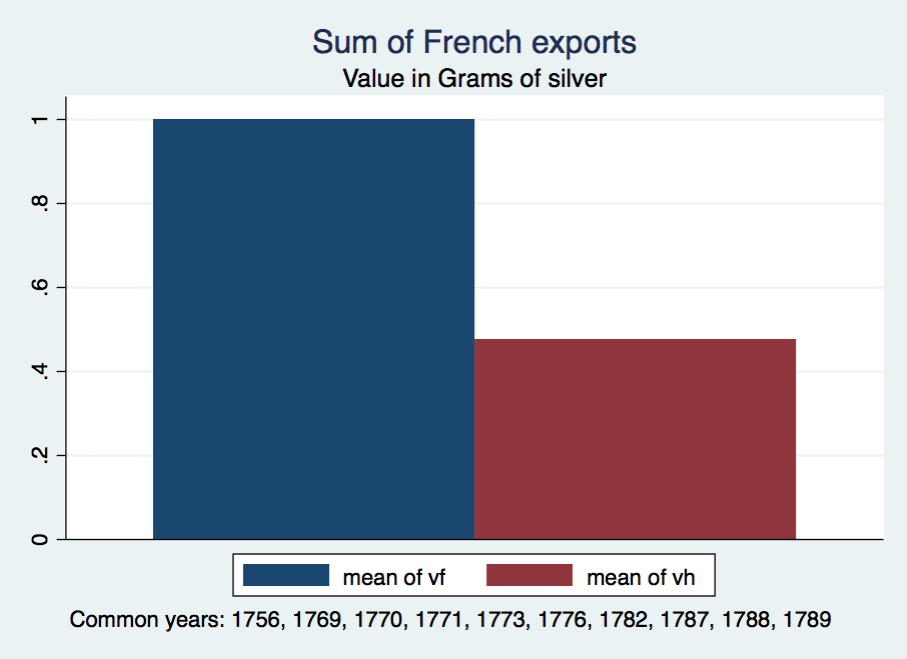
\includegraphics[scale=.28]{value_total_fr_hb_commonyears.png}
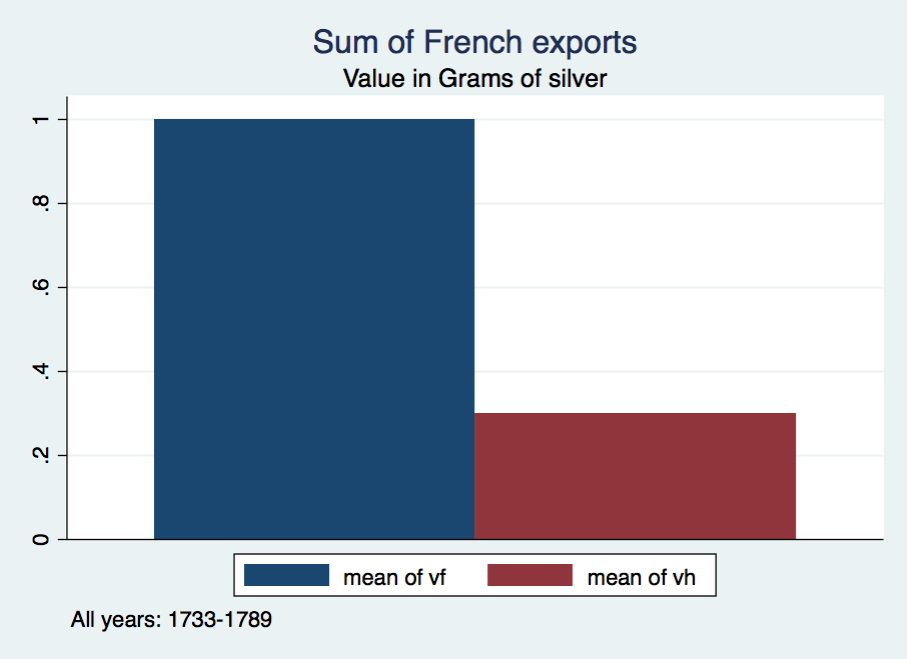
\includegraphics[scale=.28]{value_total_fr_hb.png}
Aggregate exports value in Hamburg source account for slightly less then 50\% of export value in the French source considering only common years and slightly around 30\% considering all years (1733-1789). The ratio of the two values however is far from stable; before 1740, the two sources report roughly the same value, Hamburg reports even more than France in 1735, which however might be due to the fact that the values I estimated for the period previous to 1753 for France are underestimating the real total value of exports. In the subsequent period there is a sharp decrease, and the ratio stabilizes around 5\%. Surprisingly, no major effect is evident in 1740 with the exclusion of Russia and in 1780, with the narrowing of the destination on the French dataset from “Nord” to “Hanseatic cities”. On the contrary, the ration increases. This leads me to think either to a mistake in the data, or that the share meant for Russia was only a small part of the overall export towards North.

\begin{center}
\caption{Evolution of the ratio of datasets}
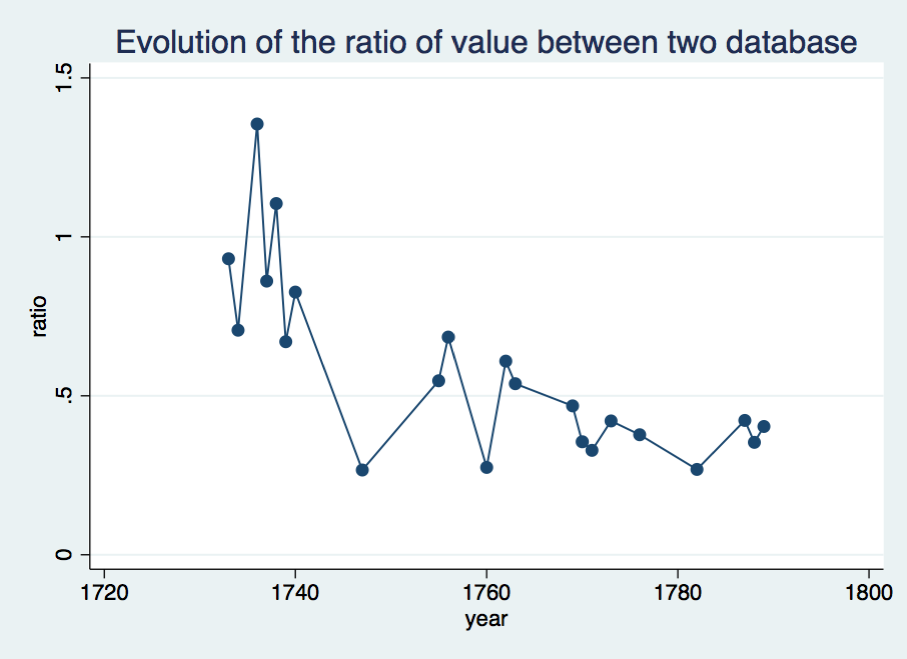
\includegraphics[scale=.3]{long_ratio.png}
\end{center}


\subsection{Comparison of total exports}
I will now turn to the evolution of aggregate exports per year.  For simplicity in comparison I have used value indexed at values in year 1787, which is the most complete for both sources. In this way I can observe better  the pattern of the two series, without considering the discrepancy in absolute value. 
From the graph below it is evident that the two sources move quite well together, with a correlation between the two series of 0.88. Also the data preceding 1740, which are an estimate, are in line with the Hamburg series. 
The overall trend of both series looks like an increasing one even though the growth is interrupted during war period. The Polish succession war between 1733 and 1738, did not seem to impact trade as much as colonial wars, whose effect on the other hand is very evident in the sharp decrease in 1761 and 1781. In this respect, I will go more into details in subsequent sections.

\begin{center}
\caption{Comparison of longitudinal evolution of aggregate exports}
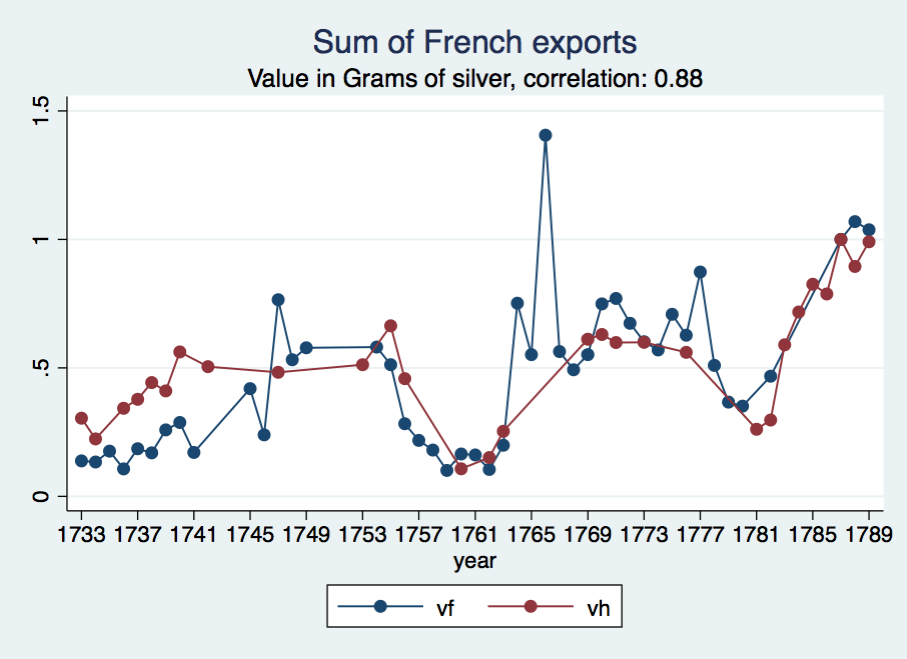
\includegraphics[scale=.3]{long_evolution.png}\\~\\
\end{center}

\subsection{Comparison at sector level}
\subsubsection{Comparison of aggregate export by sector}
The comparison at sector level brings contrasting results. At aggregate level the two sources are very close, both for the whole period and common years. It is evident that the major sector is exotic foodstuff, followed by beverages and tobacco and then by raw material, which however represents a significantly smaller share. Colonial imports are actually representing the biggest source of trade, which explains why then colonial wars were the cause of trade collapse. \\~\\
\caption{Comparison of total exports}
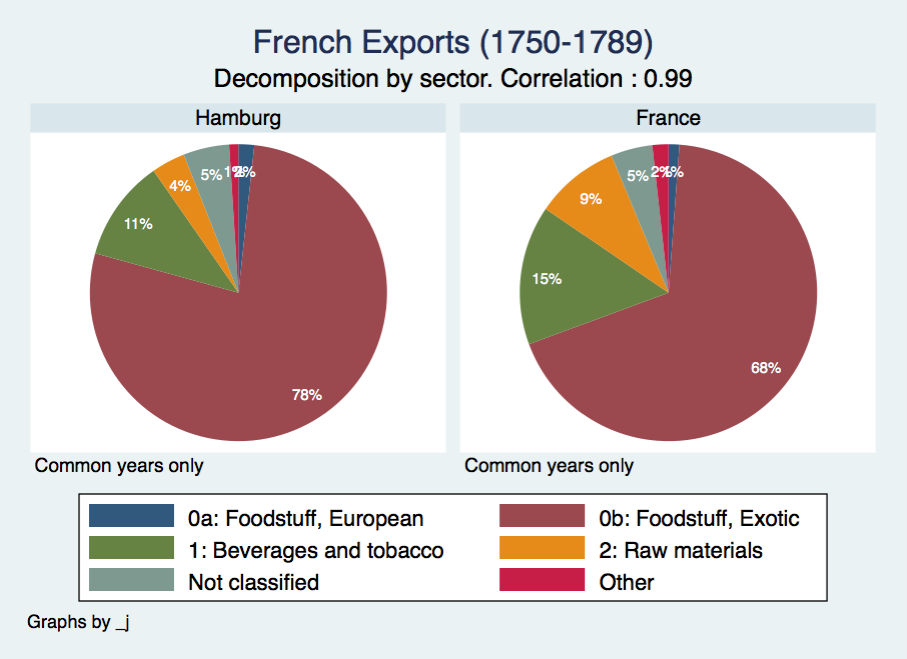
\includegraphics[scale=.28]{commonyears_sector.png}
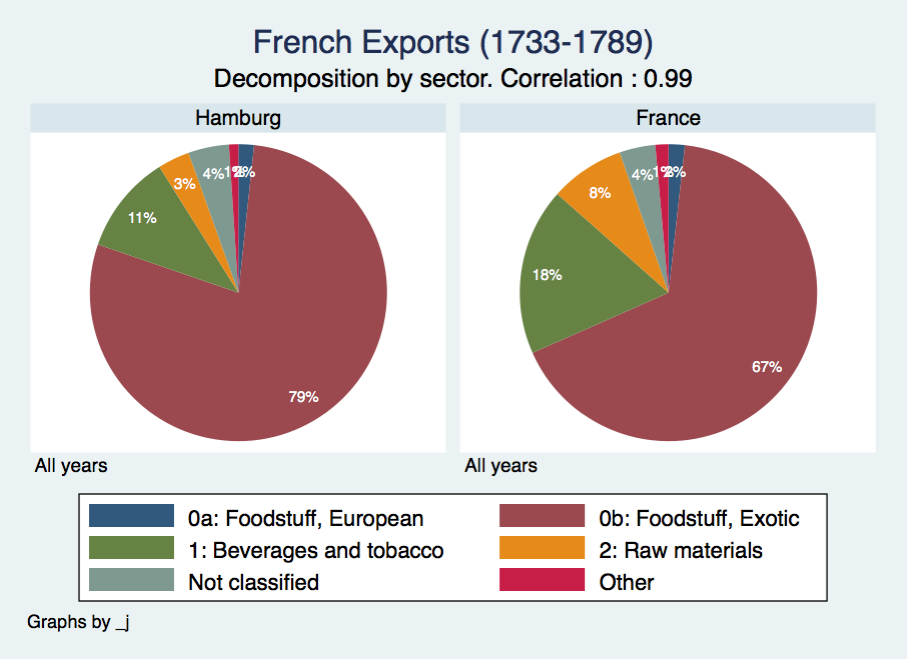
\includegraphics[scale=.28]{allyears_sector.png}

\subsubsection{Comparison of the evolution of major sectors overtime}
As mentioned above the three major sectors are Exotic foodstuffs, beverages and tobacco and raw material, with a higher importance given to the first two. The tables below plot the longitudinal evolution of these sectors according to the two different sources. Results are not as satisfactory as in the total exports longitudinal evolution above and it might be the case the estimation on the values of product pre-1750 was not too accurate because of lack of data. In all the three cases displayed below, I plotted both the share of the sector on the total and the absolute value (indexed at the 1787 value). 
\caption{Evolution of Exotic foodstuff}
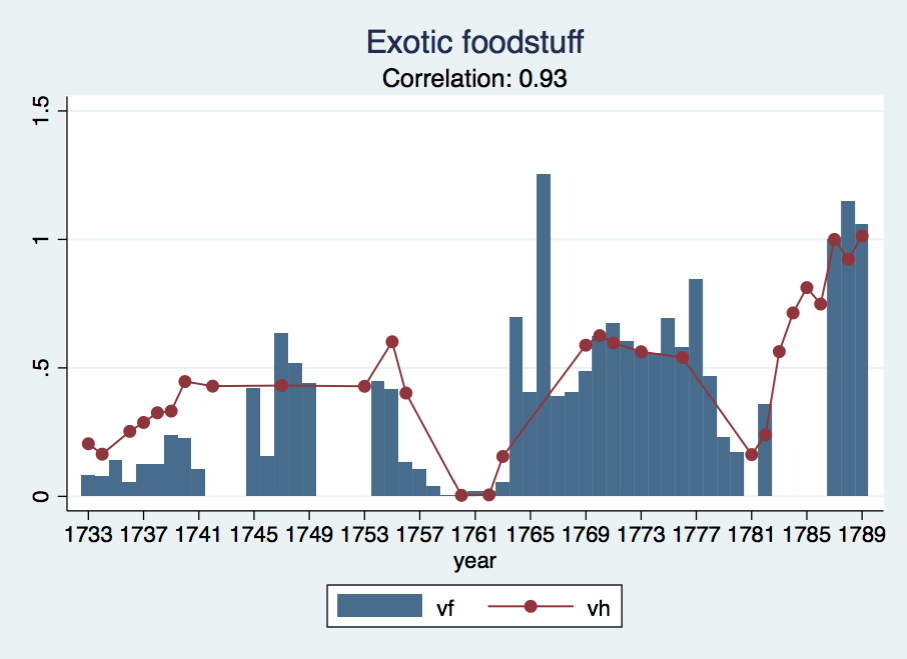
\includegraphics[scale=.28]{exotic_food_long.png}
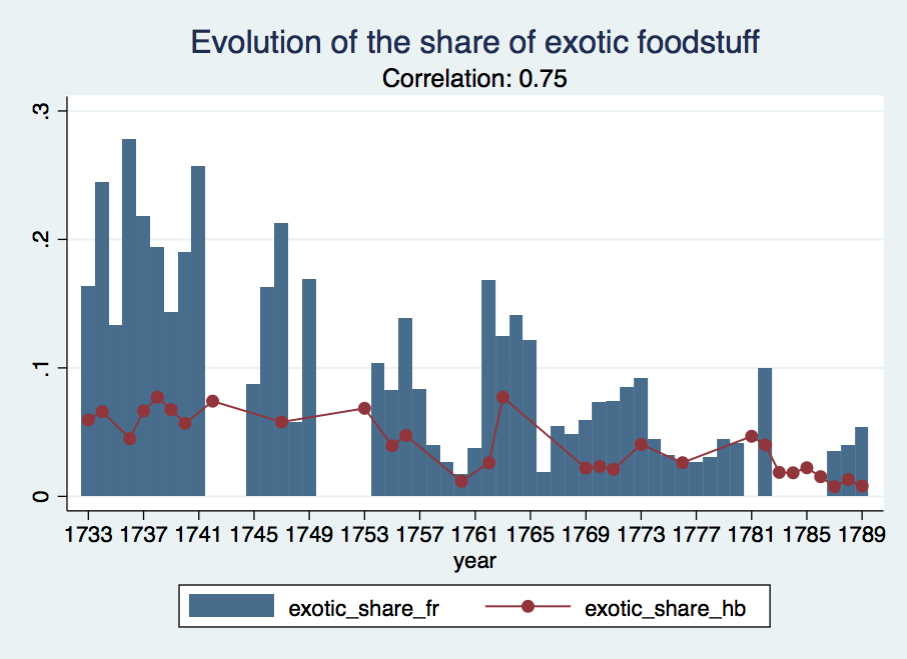
\includegraphics[scale=.28]{exotic_food_share.png}\\
\caption{Evolution of Beverages and Tobacco}
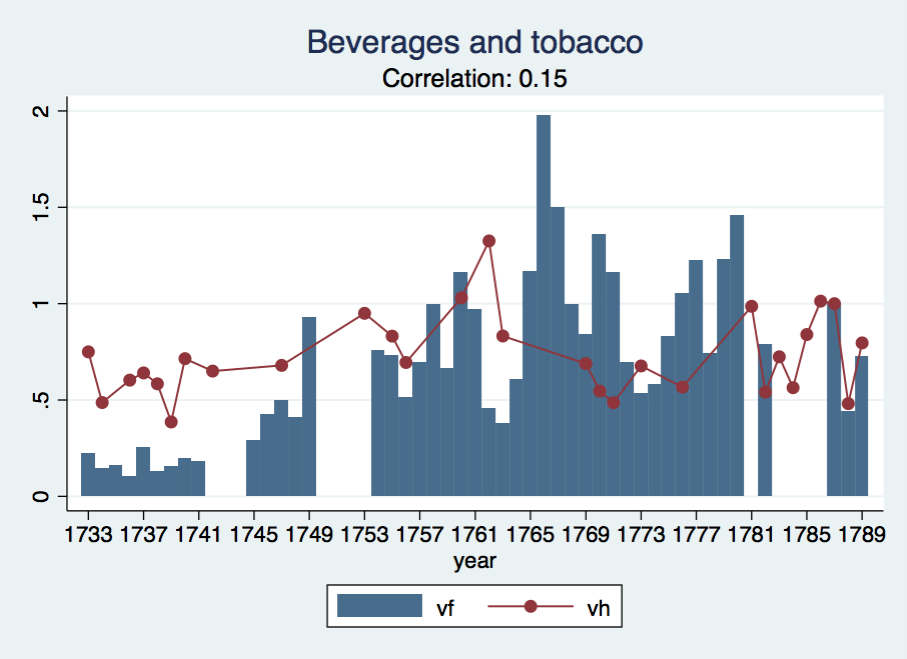
\includegraphics[scale=.28]{bev_tobacco_long.png}
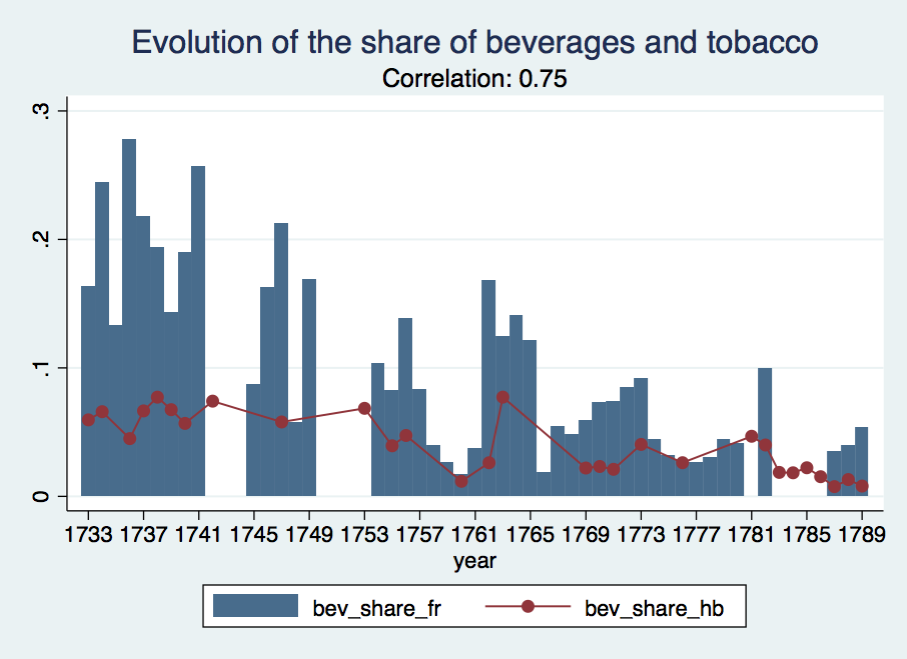
\includegraphics[scale=.28]{bev_tobacco_share.png}\\
\newpage
\caption{Evolution of Raw material}
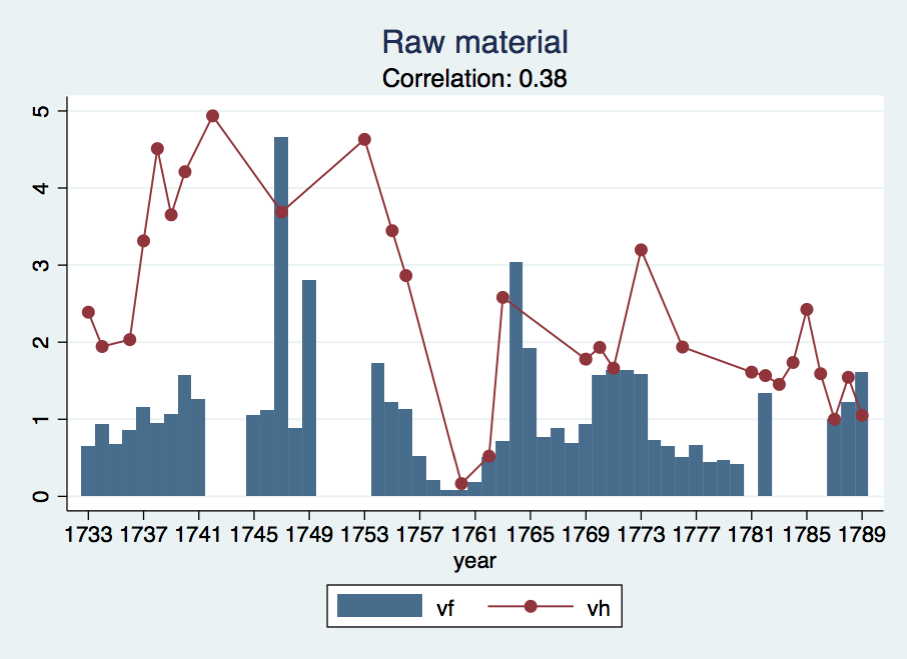
\includegraphics[scale=.28]{raw_mat_long.png}
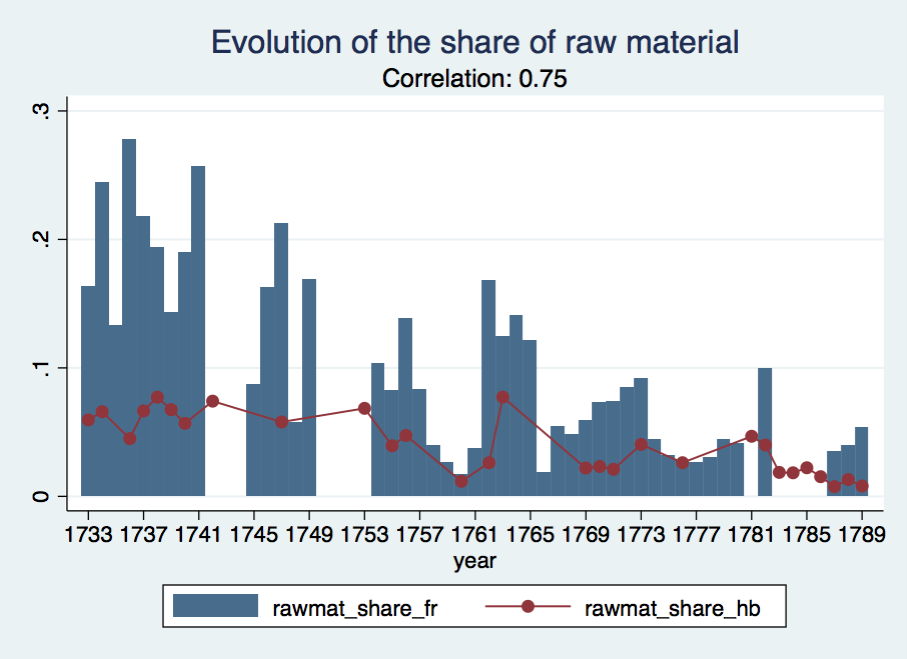
\includegraphics[scale=.28]{rawmat_share.png}

\subsection{Comparison at product}
\subsubsection{Comparison of aggregate export by product}
As for the case of sectors, products do not always give the results we would expect. At aggregate level both on all years and common years the two database are quite close:\\~\\
\caption{Evolution of coffee}
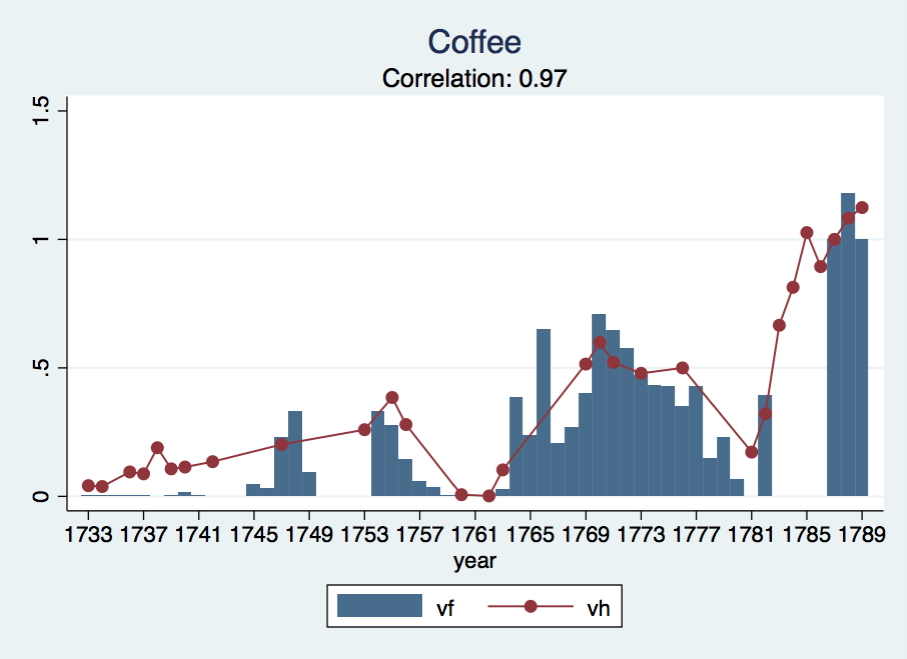
\includegraphics[scale=.28]{coffee_long.png}
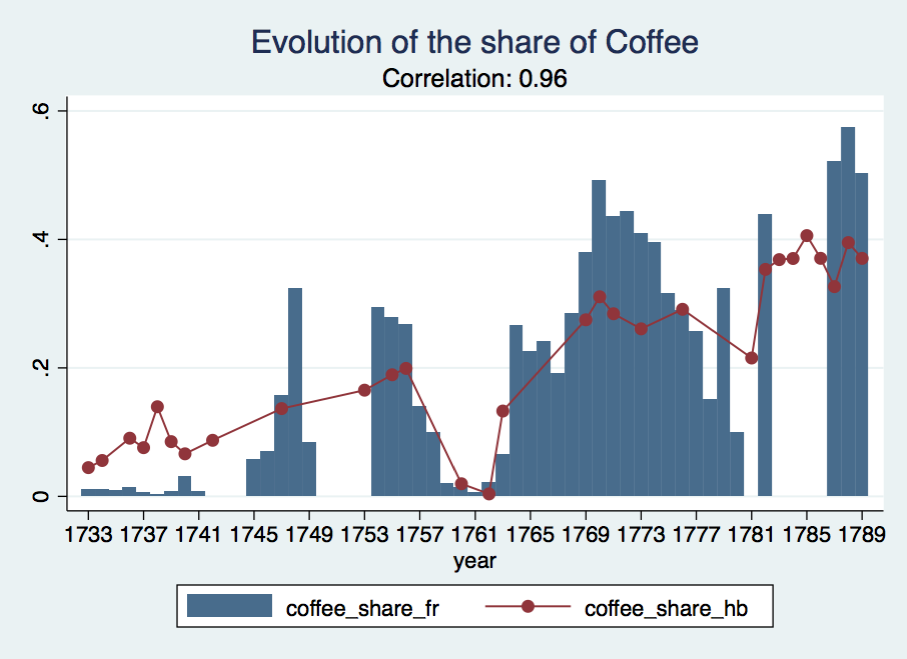
\includegraphics[scale=.28]{coffee_share_long.png}\\
\newpage
\caption{Evolution of Sugar}
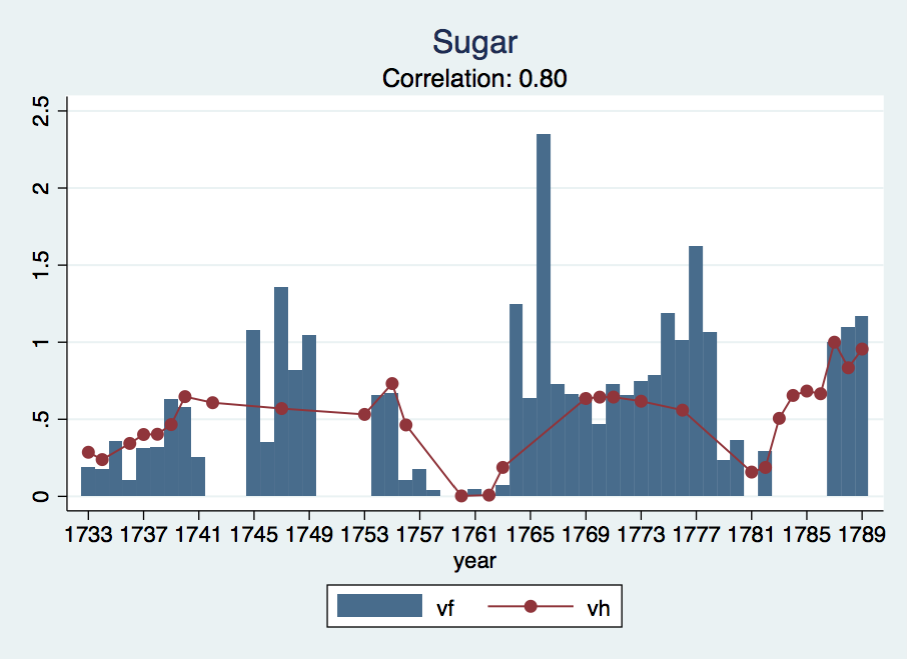
\includegraphics[scale=.28]{sugar_long.png}
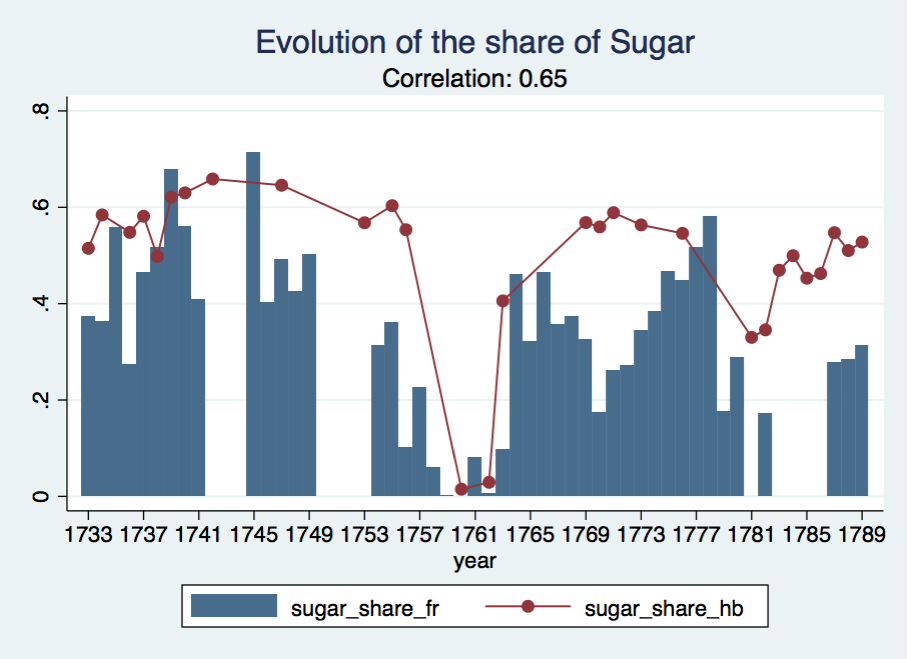
\includegraphics[scale=.28]{sugar_share_long.png}\\
\caption{Evolution of Indigo}
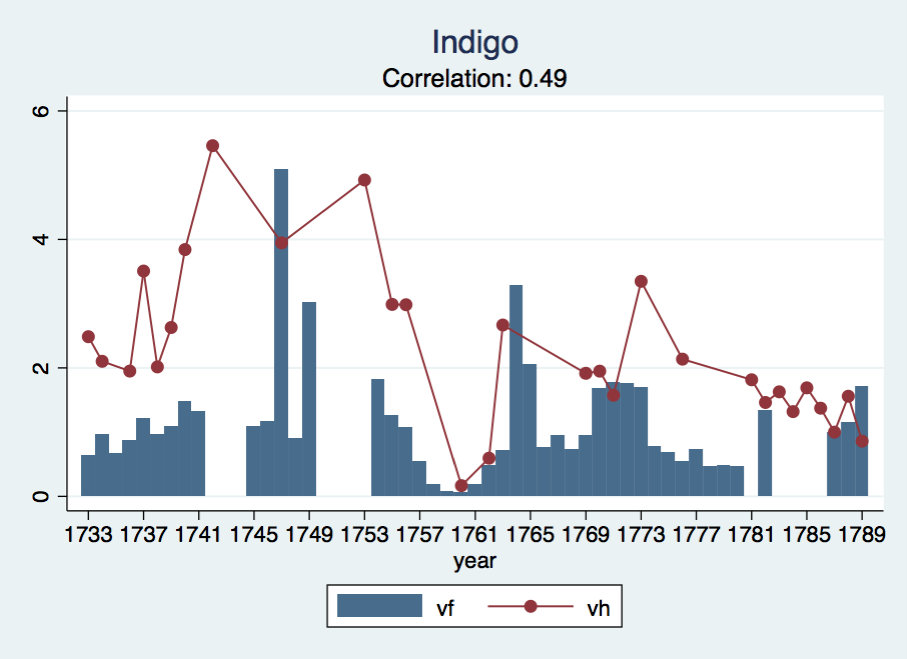
\includegraphics[scale=.28]{indigo_long.png}
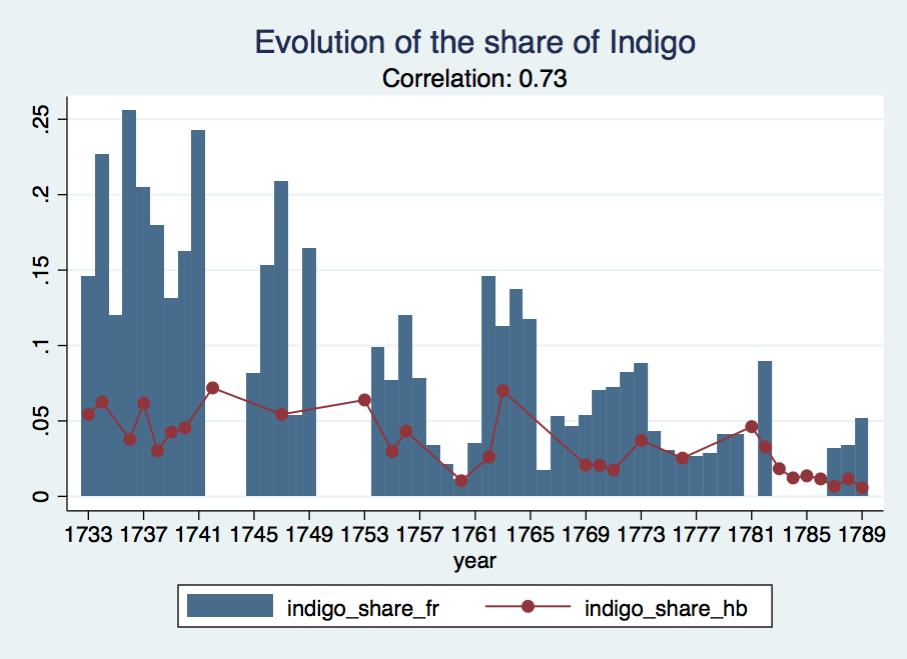
\includegraphics[scale=.28]{indigo_share_long.png}\\
\caption{Evolution of Eau de vie}
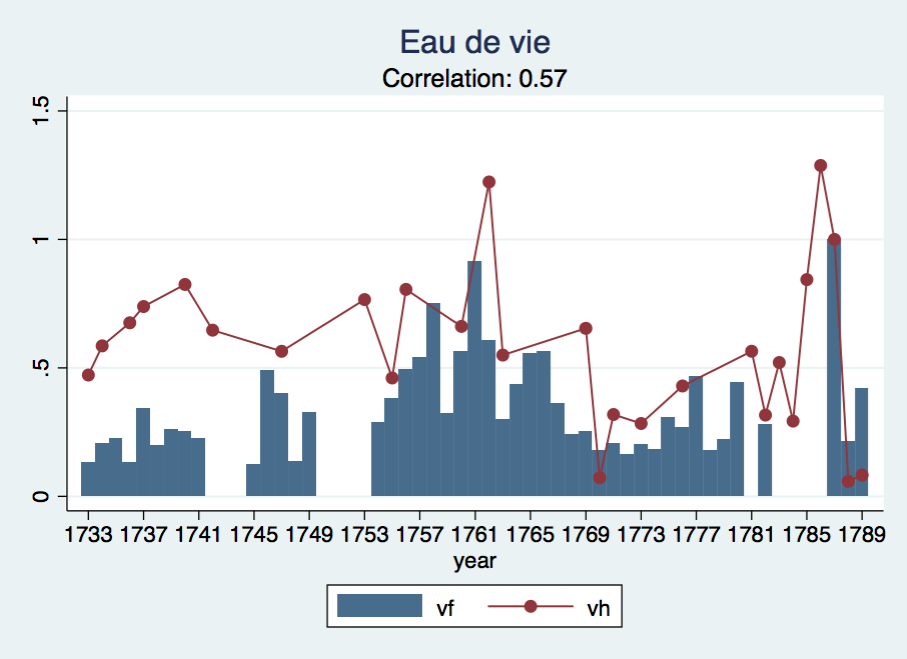
\includegraphics[scale=.28]{eaudevie_long.png}
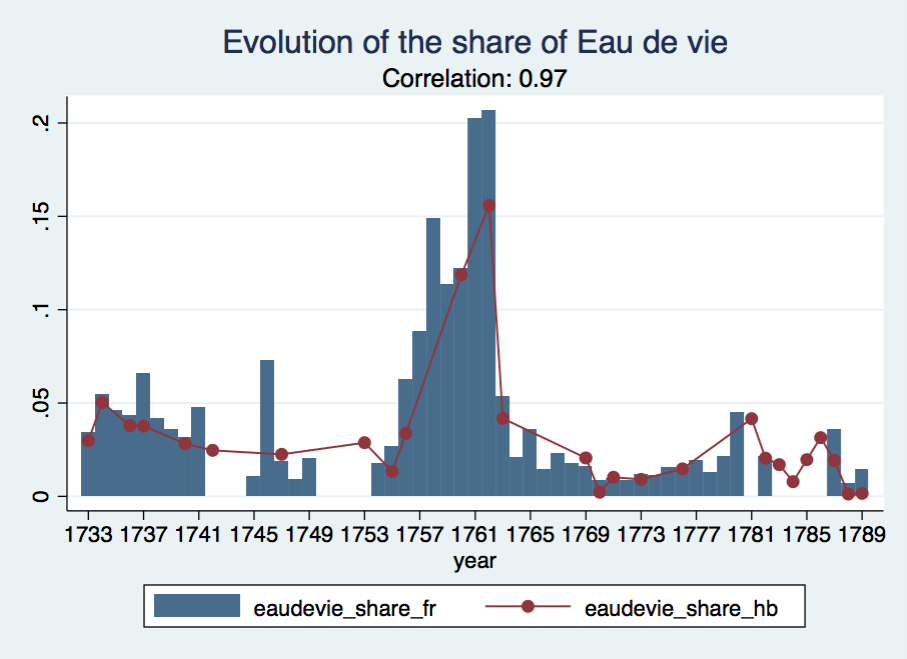
\includegraphics[scale=.28]{eaudevie_share_long.png}\\
\caption{Evolution of wine}
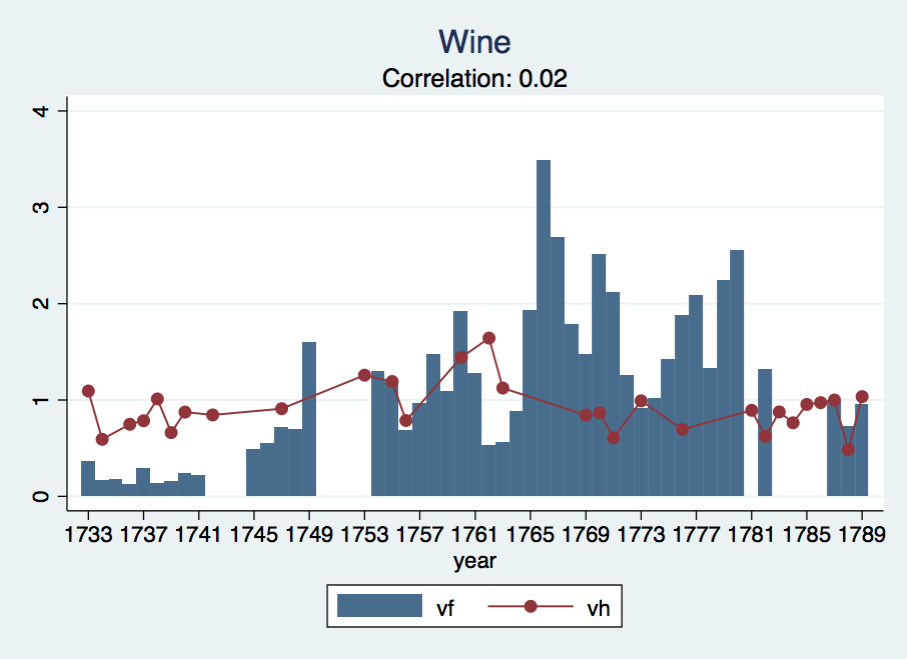
\includegraphics[scale=.28]{wine_long.png}
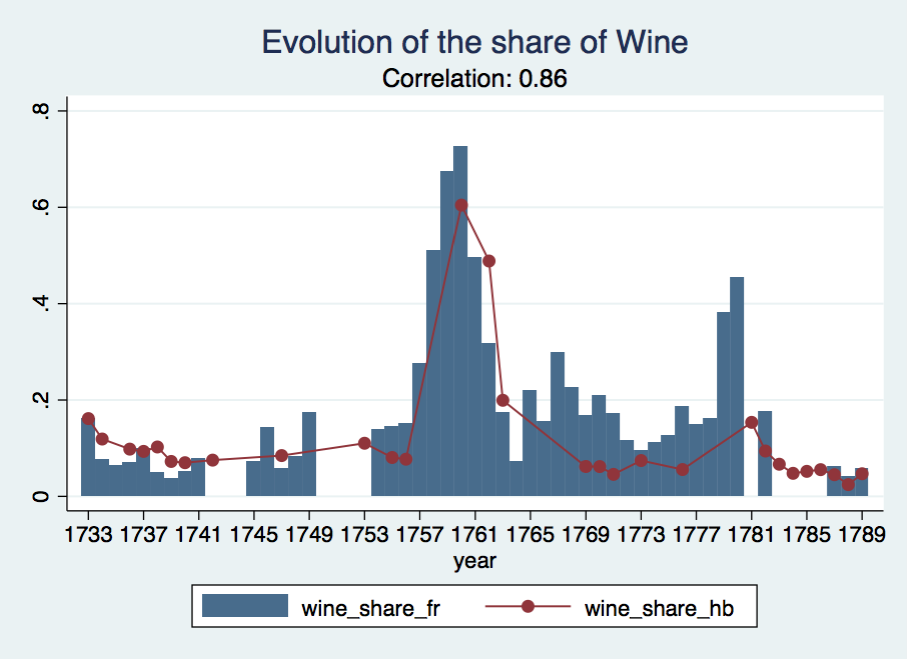
\includegraphics[scale=.28]{wine_share_long.png}
The evolution of sugar is not too precise comparing the two sources but overall the pattern is quite similar. The fact that strikes the attention is that sugar went to a nearly zero level during Seven Years War (both in share and absolute value) but experienced a less sharp decrease during the American revolutionary war. This pattern is also common to coffee and to a lesser extent to Indigo. On the contrary, in the case of wine and eau de vie, we observe an increase in export, even in absolute value, corresponding to the beginning of the Seven Years War, and then again a decline towards the end of the war. The increase in absolute value lasts till 1761 and then it also collapses together with coffee and sugar, however it remains the major source of export for the war period, especially in terms of share of overall exports. A similar pattern can be noticed during American revolutionary war but on a smaller scale. 

\subsection{Testing Benford’s law}
As a last step in my validation of the data, I have tested Benford’s law or the first-digit law on both datasets. Benford’s law is a law providing the frequency distribution of the first digit in most real life datasets. According to Benford the leading digit $d$, with $d \in \{1,...,9\}$ should follow the probability distribution: 
\begin{center}
$P(d)=\log_b(1+\frac{1}{d})$
\end{center}
where $P(d)$ is proportional to the distance between $d$ and $d+1$ on a logarithmic scale, which is the case when the logarithm of the numbers and not the numbers themselves are uniformly and randomly distributed. I run the following Pearsons’s chi square test:
\begin{center}
$$\chi^2=N\sum_{d=1}^{9}\frac{(p(d)-d(b))^2}{d(b)}$$
\end{center}
where N is the frequency and $p(d)$ and $d(b)$ are the proportions of Benford’s law and my data respectively. For both dataset I cannot reject the null hypothesis that the leading digit is actually distributed according to Benford’s law.
\caption{Benford'law}
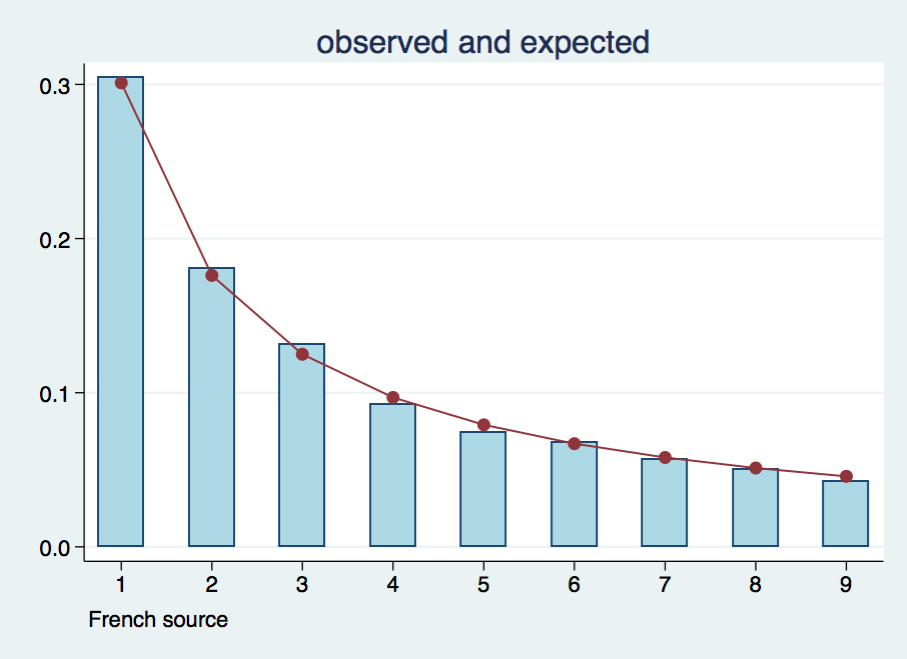
\includegraphics[scale=.28]{benford_fr.png}
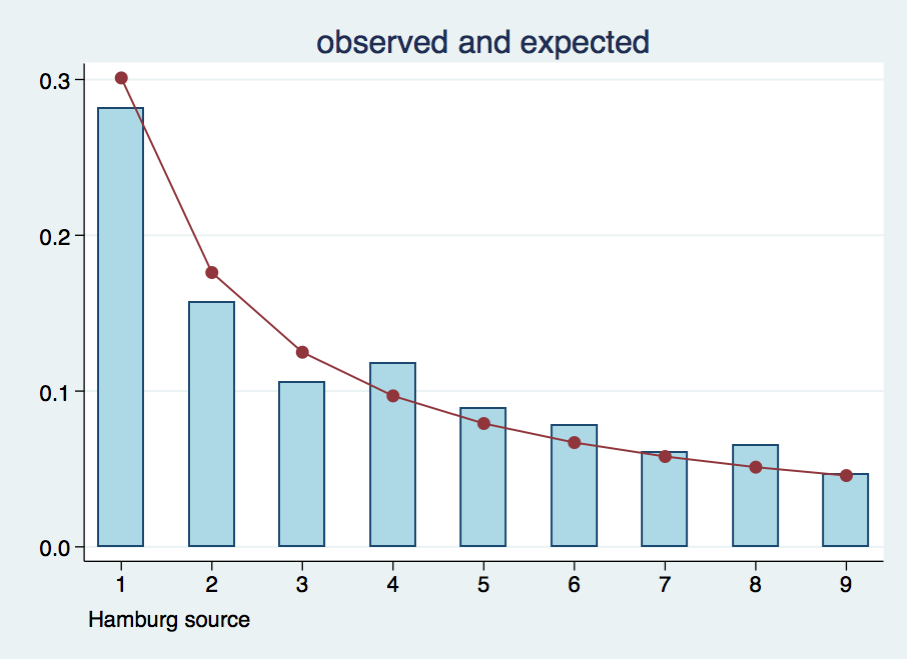
\includegraphics[scale=.28]{benford_hb.png}

\section{Analysis of trend of exports and effect of war on export for Hamburg}
From the series shown above, it is evident that trade towards Hamburg kept increasing according to both sources. However, if we look at the entire period, available only in the French dataset, the trend looks more quadratic and decreases starting 1800. 
\begin{center}
\caption{Rate of growth}
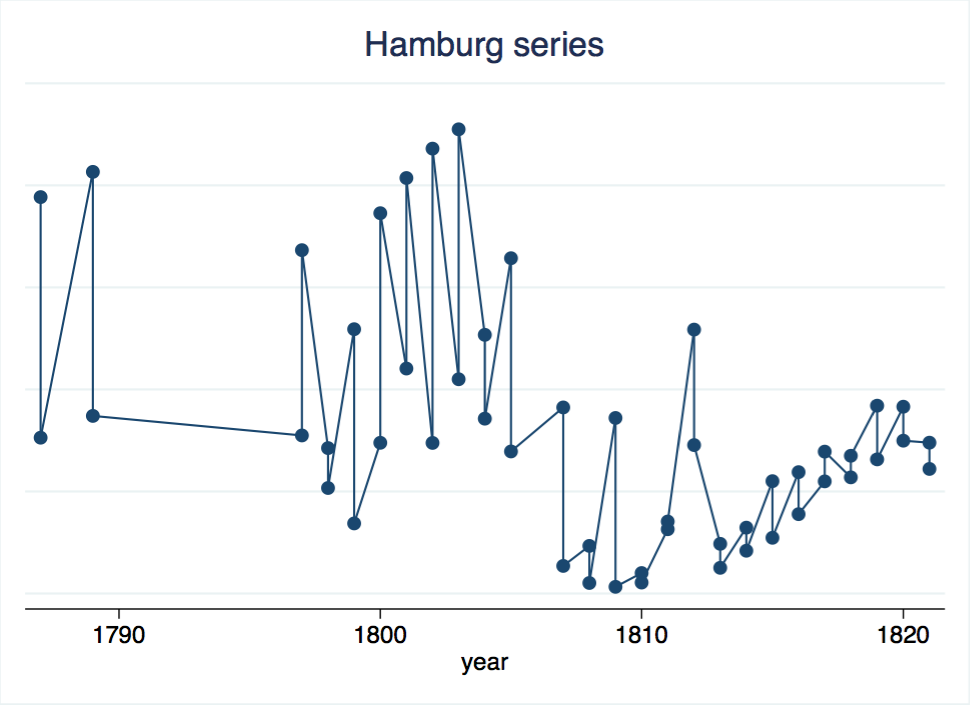
\includegraphics[scale=.3]{growth_rate.png}
\end{center}
I now want to look in details at the impact of historical events on exports, more precisely the effect of wars. There were seven major conflicts that hit Europe between 1733 and 1820; The War of the Polish succession (1733-1738), The War of the Austrian Succession (1740-1748), The Seven Years war (1756-1763), The American Revolutionary War (1775-1783), The French Revolutionary War (1792-1803) and The Napolonic War (1803-1814). The Polish succession war and the first part of the Austrian succession war were mainly fought in Europe whereas the second half of Austrian succession war (1744-1748) and the other four wars were so called colonial wars, which defined the start of a new period in eighteenth century (Carrière 1973). In all the cases, France was a belligerent country whereas Hamburg was a neutral city. So I am interested in the impact of conflicts on neutral countries in particular. Normally, neutral countries in wartime were allowed to continue their trade with all other countries, disregarding the presence of a conflict.  This rule, however, had induced belligerent countries to exploit neutral ships for trading their own merchandises (Carrière 1973). For this reason, in the beginning of Seven Years War the British decided to put an end to this practice and produced a law stating that the nationality of the ship was not relevant, but what made it or not an enemy ship was the nationality of the cargo. This fact had a considerable impact on the trade of France, who had started to use Dutch ships to transport colonial goods, but also for all other neutral countries, who were clearly showing their discontent against this new British law. Those countries, nonetheless, were not united in their protest and could not really concretize their disappointment as a unique voice. Only in 1780, a League of Armed Neutrality was created. This experiment however did not have much success in its purposes and was finally put to an end in 1783 with the treaty of Paris, when Catherina of Russia renamed it the \textit{Armed Nullity} (Griffiths, 1971). 
All this brings me to think that I should expect a strong effect of conflicts on neutral countries. 
In what follows I will give a brief description of the four conflicts and then I will proceed in the analysis of their effects on exports. 

\subsection{Historical summary}
\subsubsection{War of Polish Succession}
The war of Polish succession took place between 1733 and 1738. It started with the death of the king of Poland August II who died heirless and soon become a conflict at European level. France, Prussia and Spain were trying to limit the desire of expansion of the Habsburg monarchy, which was aiming at extend its power over Poland. The lack of support by England however, concluded the war in 1738, with the recognition of August III as king of Poland. The belligerent countries were France, Spain and Italy on the one side and the Habsburg Monarchy on the other. 

\subsubsection{War of Austrian Succession}
The war of Austrian succession was a European conflict that burst in 1740 over the eligibility to succession to the crown of Maria Theresa of Austria, as the heir of the Habsburg Monarchy after the death of her father. It started out as a European conflict but after 1744 it involved also the colonies. Belligerent countries were France, Spain, Prussia and Italy on one side and England, Habsburg monarchy and the Dutch Republic on the other. 

\subsubsection{Seven Years Wars}
The Seven year war was a major conflict, which took place between 1756 and 1763. It is consider the first real world conflict and European powers were fighting over possession of colonies. Belligerents countries were: England, Prussia and Portugal on one side and France, Spain, Habsburg monarchy, and Dutch Republic on the other. 

\subsubsection{American Revolutionary War}
The American Revolutionary War took place between 1778 and 1782. In this case the field of battle was not Europe anymore, but directly the Colonies. British North American colonies were rebelling against Britain control over their trade and were fighting for independence. Belligerent countries were England on the one side and France, Spain and British Colonies on the other (later United States). During this war the First League of Armed Neutrality was signed between Russia, Sweden and Denmark. Spain accepted this agreement however Britain demurred. When Dutch Republic was about to join this league, Britain found out before the treaty was signed and captured a Dutch ships, thus forcing the Dutch to enter war against them. Starting 1781 therefore, the Dutch Republic also became a belligerent country, allied to France. 

\subsubsection{French Revolutionary Wars}


\subsubsection{Napoleonic Wars}

\subsection{Analysis}
As a first step I have constructed a Poisson Pseudo Maximum Likelihood model with the value of exports flows towards Hamburg as a dependent variable and introducing a war dummy to capture the effect of wars. I did so first using only one dummy for all wars and then adding one dummy for each war. 
\begin{equation}
exports_t=\beta_0+\beta_1year+\beta_3year2 +\beta_4war
\end{equation}
%\begin{equation}
%\ln(exports_t)=\beta_0+\beta_1year+\beta_3polish +\beta_4austrian1 +\beta_5 austrian2 +\beta_5seven + \beta_6american
%\end{equation}

where $exports$  is the value of exports per year,  $year$ is the time trend and $year2$ is the quadratic time trend. I am using time trend rather than year fixed effects for the scarcity of data and because time fixed effects would be collinear with the war dummy otherwise.
In the case by case, I have considered the Austrian war as two different conflicts
 as to to try to capture the difference between colonial and non colonial phase.\\
From the first equation I find that wars overall had a negative impact on Hamburg trade, amounting to roughly 37\%. By breaking down the effect for each single war, I find an 8\% reduction in trade caused by the Polish war, an increase of 20\% for the first part of the Austrian war and a decrease of 22\%, 65\%, 45\%, 30\% and 34\% for the second part of Austrian war, Seven year war,  American Revolutionary war, French Revolutionary war and Napoleonic war respectively. Results are quite coherent with the series observed, with a significant drop during Seven Years war and smaller drop due to American and Napoleonic war. 
Results from the regression with no quadratic trend reveal quite contrasting effects, with the first four wars causing the major reduction in trade and the last three with a minor and insignificant results. The quadratic trend however fits the series better and I assume that results from this regression  are more accurate.
\begin{table}[htbp]\centering
\def\sym#1{\ifmmode^{#1}\else\(^{#1}\)\fi}
\caption{Hamburg Aggregate\label{tab1}}
\begin{tabular}{l*{6}{D{.}{.}{-1}}}
\toprule
                    &\multicolumn{1}{c}{No breaks}&\multicolumn{1}{c}{One break}&\multicolumn{1}{c}{Two breaks}&\multicolumn{1}{c}{No breaks}&\multicolumn{1}{c}{One break}&\multicolumn{1}{c}{Two breaks}\\
\midrule
Value               &                     &                     &                     &                     &                     &                     \\
All                 &      -0.545\sym{***}&      -0.613\sym{***}&      -0.618\sym{***}&                     &                     &                     \\
Polish              &                     &                     &                     &      -0.197         &      -0.625\sym{***}&      -0.330\sym{**} \\
Austrian1           &                     &                     &                     &      -0.818\sym{***}&      -0.207\sym{**} &      -0.876\sym{***}\\
Austrian2           &                     &                     &                     &      -0.979\sym{***}&      -0.491\sym{***}&      -1.046\sym{***}\\
Seven               &                     &                     &                     &      -0.207         &      -0.678         &      -0.678         \\
American            &                     &                     &                     &      -1.513\sym{***}&      0.0878         &      -0.102         \\
Revolutionary       &                     &                     &                     &      -0.120         &      -1.289\sym{*}  &      -1.289\sym{*}  \\
Napoleonic          &                     &                     &                     &      -1.173\sym{***}&      -1.053\sym{***}&      -1.267\sym{***}\\
\midrule
Observations        &          76         &          76         &          76         &          76         &          76         &          76         \\
Pseudo \(R^{2}\)    &       0.319         &       0.665         &       0.661         &       0.491         &       0.742         &       0.637         \\
\bottomrule
\multicolumn{7}{l}{\footnotesize \sym{*} \(p<0.05\), \sym{**} \(p<0.01\), \sym{***} \(p<0.001\)}\\
\end{tabular}
\end{table}


Looking at the figures for the pre war period, results are even more striking, trade fell by 80\%\ during the Seven Years War and by 70\%\ during American Revolutionary War. I also perform two different robustness checks for these results, using a log-linear model, (section 7) but they do not change significantly the coefficients of the regression. \\
On average we can say that wars were very disruptive for Hamburg trade, despite it being a neutral country, which does reflect what claimed by Glick and Taylor (2005), concerning effects of war even on neutral countries. One remark should be added however; wars in the first half of eighteenth century (until 1744, separation suggested by Carrière 1973), which were mostly non-colonial, had a way smaller impact on Hamburg trade. This is a first interesting result, in the sense that, we see here that not all wars had the same effects; most specifically wars fought in Europe had smaller effects than wars fought also/only in the colonies. In my opinion an explanation has to be found in the fact that the major source of import for Hamburg was actually colonial products, the trade of which during colonial wars was of course interrupted. On the other, I believe that the trade of European products did not have such a strong interruption and that it might even be the case that given the impossibility to trade exotic products, the commerce of other goods might have developed more to compensate for losses. \\
To test this hypothesis, I have looked at exports flows disaggregated by products. I only consider the main two colonial products (sugar and coffee) and the main two European products (wine and eau de vie) plus one category (other), encompassing all the remaining 35 different goods. I run the following regression, interacting the product dummies with the war dummies, first with all war together and then separately:
\begin{equation}
exports_i=\beta_0+beta_1year+\beta_2year2 + 
\beta_3product_i + \beta_4product_iyear+\beta_5product_iwar
\end{equation}

%$\ln(exports_i)=\beta_0+beta_1year+\beta_2product_i + \beta_3product_iyear+\beta_4product_ipolish + +\beta_4product_iaustrian1 + \beta_5product_iaustrian2 + \beta_6product_seven + \beta_7product_iamerican$

where$year$ and $year2$ are again the quadratic the time trend, $product_i$ is product fixed effect, $product_iyear$ is the product time trend and $product_iall$ is the interaction of the product dummy with the war dummy, which is the coefficient of interest. Table number 18 shows the results of these two regressions. \\
As I mentioned before, it is indeed the case that the impact on colonial products was significantly greater, -86\% for coffee and -67\% on sugar, whereas the impact on wine is definitely smaller and exports of eau de vie is even positive and very big in size. Looking at the time trend of each single product however, it is the case that a quadratic trend would better explain the sugar and the coffee series. For this reason I run again the same regression introducing a quadratic time trend for coffee and sugar, and I get slightly smaller figures, but still coherent signs and greater magnitude than non colonial products. \\
Given these first results, we can indeed say that the disruption in trade was led by the collapse of colonial products, but some European products, on the other hand, were even benefiting from conflicts.\\~\\
\caption{Quadratic and linear time trends}
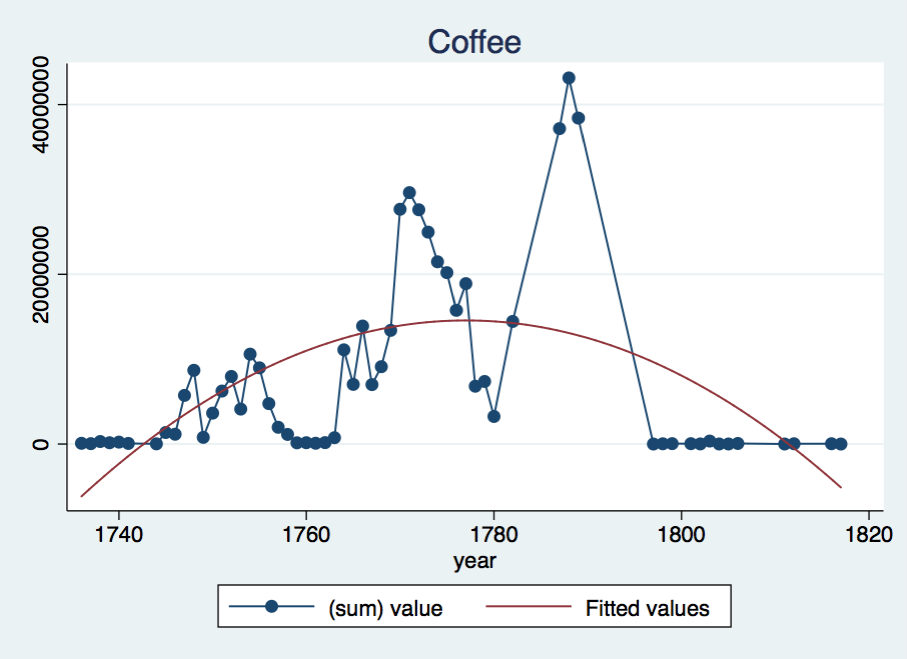
\includegraphics[scale=.28]{coffee_qfit.png}
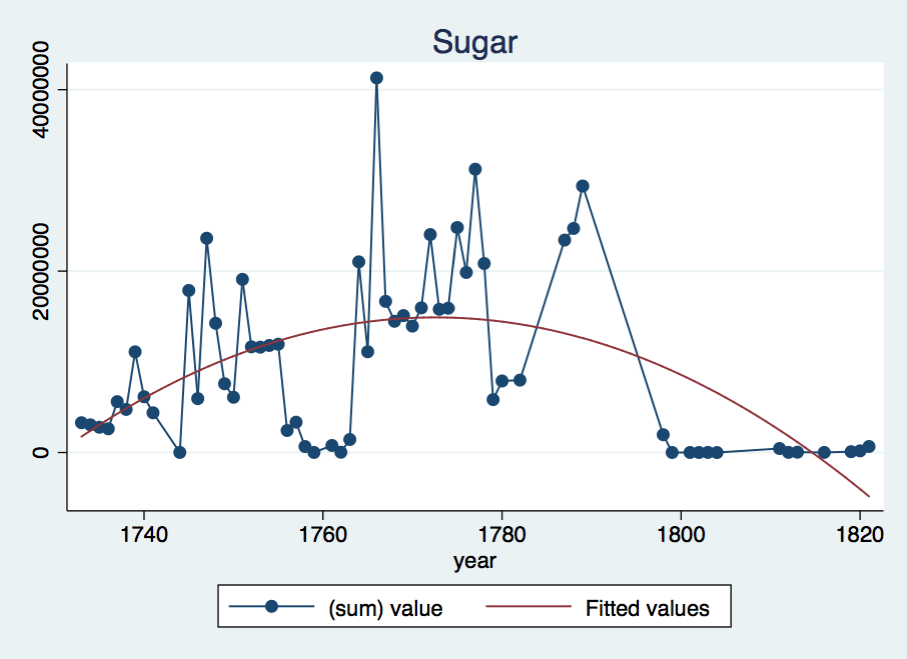
\includegraphics[scale=.28]{sugar_qfit.png}
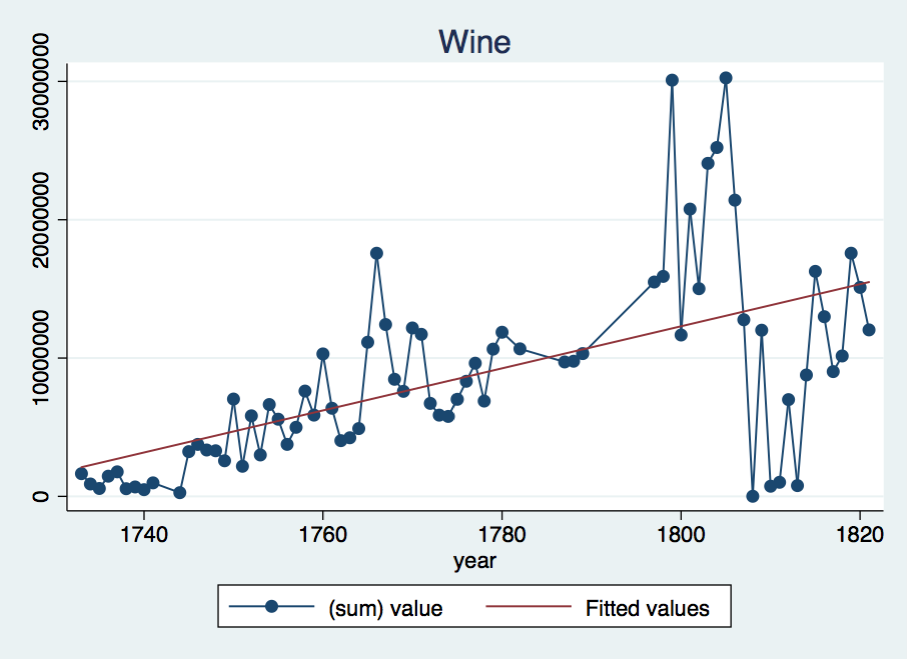
\includegraphics[scale=.28]{wine_lfit.png}
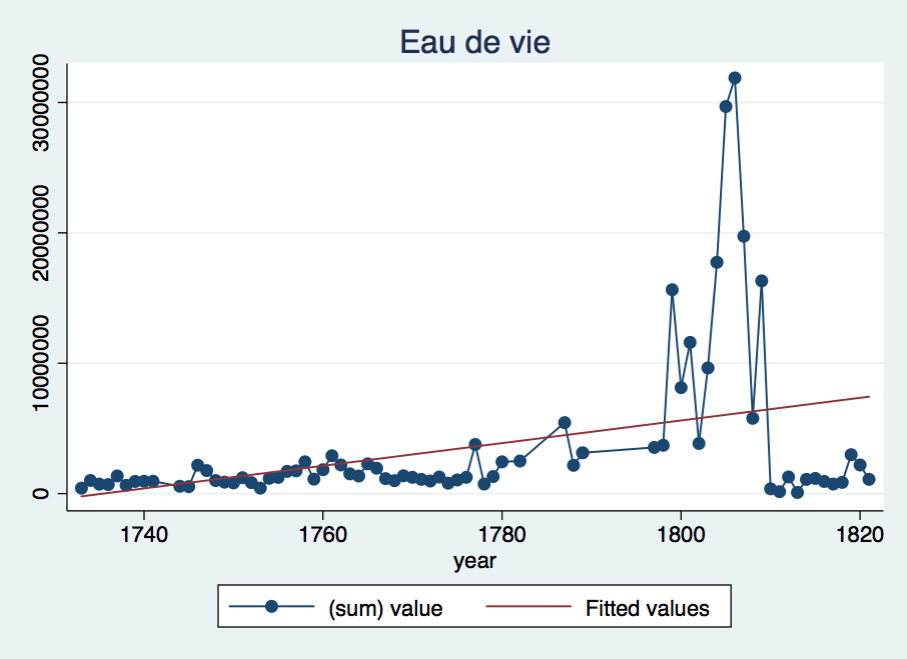
\includegraphics[scale=.28]{eau_lfit.png}\\
Turning to the war by war case, results are in line with the one-dummy for-all-wars case. The impact on coffee and sugar is very big, and it is interesting to notice that, introducing the quadratic trend for these two products, the coefficients become bigger and significant for the colonial wars, whereas it is on average smaller for the first two wars.
This is in line with my previous consideration on the difference in impact depending on the kind of war; impact is bigger on colonial products in general, but in particular during colonial conflicts. On the other hand, however, we are no more able to disentagle the colonial and non-colonial periods of the Austrian war, whose impact becomes very negative for coffee in the first part and even positive in the second, contrary to expectations. Nonetheless, it is interesting to notice that, in the case of sugar and coffee quadratic time trend, wine has a much more negative and significant coefficient for the European wars: -63\%,  -69\% and -40\% for Polish and Austrian1 and Austrian2 versus a smaller and insignificant coefficient for the subsequent wars, up to a a positive and significant impact during the Revolutionary war. 
In addition, by looking at the wine time series in section 4, we also notice an interesting pattern during Seven Years War, increasing initially and then decreasing during the second half of the conflict.  I will not analyse this issue more in detail here but it could be the object of further research. 
\begin{table}[htbp]\centering
\def\sym#1{\ifmmode^{#1}\else\(^{#1}\)\fi}
\caption{Hamburg - by product\label{tab1}}
\begin{tabular}{l*{4}{D{.}{.}{-1}}}
\toprule
                    &\multicolumn{1}{c}{All wars}&\multicolumn{1}{c}{All wars}&\multicolumn{1}{c}{War by war}&\multicolumn{1}{c}{War by war}\\
\midrule
All Coffee          &      -2.028\sym{***}&      -1.627\sym{***}&                     &                     \\
All Eau de vie      &       1.162\sym{***}&       1.192\sym{***}&                     &                     \\
All Sugar           &      -1.119\sym{***}&      -0.944\sym{***}&                     &                     \\
All Wine            &     -0.0436         &     -0.0396         &                     &                     \\
Polish Coffee       &                     &                     &      -2.865\sym{***}&      -0.746         \\
Polish Eau de vie   &                     &                     &       0.799         &      -0.334         \\
Polish Sugar        &                     &                     &      -0.523         &       0.166         \\
Polish Wine         &                     &                     &       0.246         &      -1.023\sym{**} \\
Austrian1 Coffee    &                     &                     &      -3.109\sym{***}&      -1.358\sym{*}  \\
Austrian1 Eau de vie&                     &                     &       0.599         &      -0.272         \\
Austrian1 Sugar     &                     &                     &      -0.454         &      0.0531         \\
Austrian1 Wine      &                     &                     &      -0.663         &      -1.658\sym{***}\\
Austrian2 Coffee    &                     &                     &      -0.421         &       0.793         \\
Austrian2 Eau de vie&                     &                     &       0.482         &      -0.124         \\
Austrian2 Sugar     &                     &                     &       0.125         &       0.450         \\
Austrian2 Wine      &                     &                     &       0.205         &      -0.507\sym{*}  \\
Seven Coffee        &                     &                     &      -2.315\sym{***}&      -2.048\sym{***}\\
Seven Eau de vie    &                     &                     &       0.282         &       0.177         \\
Seven Sugar         &                     &                     &      -2.627\sym{***}&      -2.607\sym{***}\\
Seven Wine          &                     &                     &      0.0224         &      -0.147         \\
American Coffee     &                     &                     &      -1.037\sym{***}&      -1.293\sym{***}\\
American Eau de vie &                     &                     &      -0.271         &   -0.000709         \\
American Sugar      &                     &                     &      -0.618\sym{*}  &      -0.713\sym{*}  \\
American Wine       &                     &                     &      -0.287\sym{*}  &     -0.0241         \\
Napoleonic Coffee   &                     &                     &      -5.484\sym{***}&      -4.837\sym{***}\\
Napoleonic Eau de vie&                     &                     &       2.088\sym{***}&       2.115\sym{***}\\
Napoleonic Sugar    &                     &                     &      -4.313\sym{***}&      -3.882\sym{***}\\
Napoleonic Wine     &                     &                     &      -0.154         &     -0.0532         \\
Revolutionary Coffee&                     &                     &      -6.693\sym{***}&      -6.460\sym{***}\\
Revolutionary Eau de vie&                     &                     &       1.422\sym{***}&       1.622\sym{***}\\
Revolutionary Sugar &                     &                     &      -3.154\sym{***}&      -2.947\sym{***}\\
Revolutionary Wine  &                     &                     &       0.127         &       0.379\sym{*}  \\
Cons                &     -1634.2\sym{***}&     -6756.7\sym{***}&     -2589.6\sym{***}&     -6698.1\sym{***}\\
Product FE          &         Yes         &         Yes         &         Yes         &         Yes         \\
Product time trend  &         Yes         &         Yes         &         Yes         &         Yes         \\
Quadratic trend     &         Yes         &         Yes         &         Yes         &         Yes         \\
Product quadratic trend&          No         &         Yes         &          No         &         Yes         \\
\midrule
Observations        &         347         &         347         &         347         &         347         \\
Pseudo \(R^{2}\)    &       0.535         &       0.593         &       0.678         &       0.720         \\
\bottomrule
\multicolumn{5}{l}{\footnotesize \sym{*} \(p<0.05\), \sym{**} \(p<0.01\), \sym{***} \(p<0.001\)}\\
\end{tabular}
\end{table}

In sum, from the estimations made so far, we can conclude that there was indeed a negative impact on neutral countries, but which was mainly concentrated on colonial products. 

The impact on European products was found strongly negative for European wars but not that significant in Colonial wars. These results are already in contrast with some of the literature (i. e. Glick and Taylor (2005) and Thierry, Martin and Mayer (2010)), which found generic negative impact on trade with no war-type or product-type differentiation. Only Blomberg and Hess (2004), have disentangled the impact of different kind of conflicts but they focused on external versus internal violence instead.\\
Another interesting issue which is extensively treated in the literature is the presence of war lags and slow trade recovery after conflicts. Glick and Taylor (2005) for instance, found major war lags for both neutral and adversary countries for a period up to ten years. I have tested their findings on my Hamburg series, adding to the above regressions dummies for lag from 1 to 5 years (tables are the appendix). I have opted for 5 years of lag because in this period trade was much more unstable and effects after five years might have been due to other unrelated issues. In addition, using 10 years lags would basically mean including another war period. For this same reason I am only looking at lags for the Austrian Succession war, Seven Years War and Napoleonic wars, and those three wars together (no data are available for the period immediately after American Revolutionary War). I have done so again on all wars together and on wars separately as before. Results are not very coherent across regressions. In the overall case, coefficients of lag dummies are negative but alternate in  sign and size, with the first year of lag being insignificant. Splitting the one war dummy into the five different wars, we do not find more revealing results; lags are alternating positive and negative coefficients, with the only exception of the Austrian war, which shows a positive and negative coefficient from the the first year after the war. Turning to the breakdown by product, we notice that there is evidence of war lags for coffee up to three years and to a minor extent on sugar, which has a two negative lags, after experiencing an increase. Wine has a very small coefficient, which becomes even positive on the second year of lag and finally eau de vie has 5 years of negative lags, however coefficients are never significant. In the war by war case, results are even less coherent, with stable figures only for coffee, which shows again 3 years of lagged effects of war. \\~\\
****\\
Overall we can say than rather than a war lag we see an increase of exports at the end of the war. This was also noted by Riley (1984), who analyses the case of the Seven Years War and claims that merchants were actually forecasting the wars (using price of lead) and stocking products to sell them at the end of the conflict, thus compensating for war losses. He also claims that this was not only happening after the wars but also before, so he saw an increase in exports before and after wars. I have tested his findings on my data by adding to the main regression a dummy for up to four years preceeding the conflict, as suggested by Riley (1984). In the general case (all wars in one dummy) coefficient are positive but very small, so Riley’s claim is not really reflected here. On the other hand, in the war-by-war case, coefficients for one year preceding conflict are positive and bigger in size, however it is not a constant effect throughout the four years. 
I have then run the same regressions by adding product fixed effects, as before, and introducing pre-war dummies interacted with products. Results do not differ much from the aggregate level; there is a constant positive effect one year before the war, which in this case it is more pronounced for European goods. In the war-by-war case finally, there is no big change with the results of the other regressions. \\
In short, I have found no evidence of war lags or loss in trade subsequent to the war, it looks more like trade increased after the war (all coefficient are positive) and even if it does not exactly overshoot, at least it recovered extremely fast its pre-war level and growth rate. 
In this section I have made four main points on the impact of war on Hamburg; 1) war is indeed a major source of trade disruption, 2) the impact however was mainly on colonial goods such as sugar and coffee, 3) there is no evidence of war lags but on the contrary trade increased following the conflict 4) It was not possible to disentangle precisely the effect of colonial versus non colonial wars. In next section I compare these findings with the case of overall exports of France towards all countries. \\
*****
\section{Comparison with French total exports}
In this section I have compared the results obtained for Hamburg with the general case of all French trading partners in eighteenth century. I have run a difference in difference specification to see the difference in impact for neutral and adversary countries with respect to allies. As for Hamburg, I have again incomplete data on products preceding 1750, so I have estimated the value for sugar coffee, wine and eau de vie through the same technique. \\
I started my analysis running the following equation for all wars together and separately:
\begin{equation}
exports_{i,t}=\beta_0+\beta_1year + \beta_2country_i+\beta_3country_iyear+\beta_4adversaries_i+\beta_5neutral_i
\end{equation}

where $year$ is year time trend, $country$ is country fixed effects, $country_iyear$ is country time trends, $adversaries$ is a dummy variable that takes value 1 if a country is adversary to France during a conflict and $neutral$ is again a dummy indicating whether a country was neutral (rather than adversary or allied). Even in this case I did not have enough data to estimate country year fixed effects so I have used time trend.\\
From the first regression we can see that war had on average a negative impact on trade of neutral countries of around 22\%. As for the case of Hamburg, I have added a non linear time trend for some countries, namely Spain, Flanders, Netherlands, Italy, Levant, North, Switzerland and United States. Series with quadratic and linear fit are to be found in the appendix. 
By looking at each single war, we notice that the difference in impact between colonial and non colonial war is not as more evident. Without considering the quadratic trend of certain countries, the Polish war is the most disruptive. However, once we account for the non linearity, this coefficient is reduced, remaining however the third strong impact found in the war by war case. We notice also that the last two wars are quite small in their impact and non significant.
Overall the impact for all wars is indeed negative and this finding is line with Hamburg case, discussed previously. However loss estimated for neutral countries are by far less striking than the ones found looking at the Hamburg series. Even though the sign of the coefficients expressing the war effect is the same, there is an evident stronger effect in the Hamburg case. For this reason I have looked again into the breakdown by the major products and analysed the impact of wars on different goods. I am arguing that in eighteenth century wars did not have an impact on all goods, but rather on some specific goods. Hamburg imports from France were mainly made up of colonial products, which were more vulnerable to conflicts, and this explains why its losses were so huge. On the other hand, this was not the case for other countries, whose import composition was totally different and which probably suffered to a lesser extent. Different destinations had really different patterns of exports, and it would be interesting to see whether groups of nations suffered more according to their import composition than their belligerent/neutral status. 
In this setting, however, I am only considering the four main goods analysed in the Hamburg case, as to be able to perform a comparison.\\
More than an impact on all trade, I believe it was a matter of impact on trade of certain products. \\
In line with this reasoning, I run again a regression with a product breakdown and analyse the impact of all conflicts together and war by war:
\begin{multline}
exports_{i,t}=\beta_0+\beta_1year +\beta_2country_i+\beta_3country_iyear+\beta_4product_{i,j}+\beta_5product_jyear+\\+\beta_6product_jadversary + \beta_7product_jneutral
\end{multline}
where $country_iproduct_j$ is country product fixed effects, $country_iyear$ and $product_jyear$ are country and product time trend and $product_jadversary$ and $product_jneutral$ are adversaries and neutral dummies interacted with product dummies. This regression lies on the assumption that product fixed effects are country-specific whereas product time trend do not differ across countries. I have also run a specification where I relax this assumption and I assumes both country products fixed effects and country products specific trends, but the difference is not noticeable (section 7). 

\begin{table}[htbp]\centering
\def\sym#1{\ifmmode^{#1}\else\(^{#1}\)\fi}
\caption{ALL COUNTRIES: Aggregate\label{tab1}}
\begin{tabular}{l*{4}{D{.}{.}{-1}}}
\hline\hline
                    &\multicolumn{1}{c}{All wars}&\multicolumn{1}{c}{Quadratic}&\multicolumn{1}{c}{Quadratic}&\multicolumn{1}{c}{War by war}\\
\hline
Adversary           &      -0.324\sym{***}&      -0.254\sym{***}&                     &                     \\
Neutral             &      -0.283\sym{***}&      -0.245\sym{***}&                     &                     \\
Polish adversary    &                     &                     &      -0.859\sym{***}&       1.601\sym{***}\\
Austrian1 adversary &                     &                     &     -0.0507         &       0.367\sym{**} \\
Austrian2 adversary &                     &                     &      -0.334\sym{*}  &    -0.00678         \\
Seven adversary     &                     &                     &      -0.827\sym{***}&      -0.728\sym{***}\\
Napoleonic adversary&                     &                     &      -0.168         &      -0.165         \\
Revolutionary adversary&                     &                     &      -1.114\sym{***}&      -1.112\sym{***}\\
Polish neutral      &                     &                     &      -0.803\sym{***}&      -0.342\sym{***}\\
Austrian1 neutral   &                     &                     &      -0.329\sym{***}&      0.0524         \\
Austrian2 neutral   &                     &                     &      -0.499\sym{***}&      -0.231\sym{***}\\
Seven neutral       &                     &                     &      -0.515\sym{***}&      -0.494\sym{***}\\
American neutral    &                     &                     &      -0.137         &      -0.357\sym{***}\\
Napoleonic neutral  &                     &                     &      -0.171         &      -0.155         \\
Revolutionary neutral&                     &                     &     -0.0914         &      -0.147         \\
Constant                &      -21.57\sym{***}&      -21.10\sym{***}&      -20.23\sym{***}&      -20.36\sym{***}\\
Country FE          &         Yes         &         Yes         &         Yes         &         Yes         \\
Country time trend  &         Yes         &         Yes         &         Yes         &         Yes         \\
Country quadratic trend&          No         &         Yes         &          No         &         Yes         \\
\hline
Observations        &         836         &         836         &         836         &         836         \\
Pseudo \(R^{2}\)    &       0.710         &       0.756         &       0.737         &       0.784         \\
\hline\hline
\multicolumn{5}{l}{\footnotesize \sym{*} \(p<0.05\), \sym{**} \(p<0.01\), \sym{***} \(p<0.001\)}\\
\end{tabular}
\end{table}

\begin{table}[htbp]\centering
\def\sym#1{\ifmmode^{#1}\else\(^{#1}\)\fi}
\caption{ALL COUNTRIES: all wars by product\label{tab1}}
\begin{tabular}{l*{4}{D{.}{.}{-1}}}
\hline\hline
			  &\multicolumn{1}{c}{All wars}&\multicolumn{1}{c}{All wars}&\multicolumn{1}{c}{All wars}\\
\hline
Adversary Coffee    &      -1.170\sym{*}  &      -0.207         &      -1.123\sym{*}  \\
Adversary Eau de vie&      0.0514         &      0.0511         &      0.0698         \\
Adversary Sugar     &      -2.030\sym{***}&      -2.030\sym{***}&      -1.962\sym{***}\\
Adversary Wine      &       0.283\sym{**} &       0.283\sym{**} &       0.323\sym{**} \\
Neutral Coffee      &      -1.695\sym{***}&      -1.289\sym{***}&      -1.619\sym{***}\\
Neutral Eau de vie  &       0.756\sym{***}&       0.756\sym{***}&       0.752\sym{***}\\
Neutral Sugar       &      -1.448\sym{***}&      -1.448\sym{***}&      -1.382\sym{***}\\
Neutral Wine        &     -0.0898         &     -0.0898         &     -0.0854         \\
Constant            &      -25.55\sym{**} &     -5380.4\sym{***}&      -23.71\sym{**} \\
Country-product FE  &         Yes         &         Yes         &         Yes         \\
Country time trend  &         Yes         &         Yes         &         Yes         \\
Product time trend  &         Yes         &         Yes         &         Yes         \\
Country quadratic trend&          No         &          No         &         Yes         \\
Product quadratic trend&          No         &         Yes         &          No         \\
\hline
Observations        &        3130         &        3130         &        3130         \\
Pseudo \(R^{2}\)    &       0.743         &       0.747         &       0.747         \\
\hline\hline
\multicolumn{4}{l}{\footnotesize \sym{*} \(p<0.05\), \sym{**} \(p<0.01\), \sym{***} \(p<0.001\)}\\
\end{tabular}
\end{table}

\begin{table}[htbp]\centering
\def\sym#1{\ifmmode^{#1}\else\(^{#1}\)\fi}
\caption{ALL COUNTRIES:Each war by product\label{tab1}}
\begin{tabular}{l*{3}{D{.}{.}{-1}}}
\hline\hline
                    &\multicolumn{1}{c}{All wars}&\multicolumn{1}{c}{All wars}&\multicolumn{1}{c}{All wars}\\
\hline
Polish neutral Eau de vie&       0.593\sym{*}  &       0.594\sym{*}  &       1.061\sym{***}\\
Polish neutral Sugar&      -2.078\sym{***}&      -2.077\sym{***}&      -1.873\sym{**} \\
Polish neutral Wine &       0.131         &       0.131         &       0.602\sym{*}  \\
Austrian1 neutral Eau de vie&      -0.153         &      -0.153         &       0.370\sym{*}  \\
Austrian1 neutral Sugar&      -2.198\sym{**} &      -2.197\sym{**} &      -2.025\sym{*}  \\
Austrian1 neutral Wine&      -1.769\sym{***}&      -1.769\sym{***}&      -1.229\sym{***}\\
Austrian2 neutral Coffee&      -0.746\sym{*}  &       1.195\sym{**} &       1.214\sym{**} \\
Austrian2 neutral Eau de vie&     0.00109         &     0.00115         &       0.331         \\
Austrian2 neutral Sugar&      -0.798         &      -0.797         &      -0.679         \\
Austrian2 neutral Wine&      -0.593\sym{*}  &      -0.593\sym{*}  &      -0.246         \\
Seven neutral Coffee&      -2.034\sym{***}&      -1.588\sym{***}&      -1.606\sym{***}\\
Seven neutral Eau de vie&       0.544\sym{**} &       0.545\sym{**} &       0.562\sym{**} \\
Seven neutral Sugar &      -1.266\sym{*}  &      -1.266\sym{*}  &      -1.266\sym{*}  \\
Seven neutral Wine  &      0.0816         &      0.0825         &       0.128         \\
American neutral Coffee&      -0.479\sym{*}  &      -1.028\sym{***}&      -1.050\sym{***}\\
American neutral Eau de vie&      0.0448         &      0.0458         &      -0.236         \\
American neutral Sugar&      -0.801         &      -0.801         &      -0.912\sym{*}  \\
American neutral Wine&     -0.0337         &     -0.0328         &      -0.279\sym{*}  \\
Napoleonic neutral Coffee&      -2.810\sym{***}&      -2.156\sym{***}&      -2.112\sym{***}\\
Napoleonic neutral Eau de vie&       0.951\sym{***}&       0.951\sym{***}&       0.950\sym{***}\\
Napoleonic neutral Sugar&      -4.276\sym{***}&      -4.276\sym{***}&      -4.195\sym{***}\\
Napoleonic neutral Wine&      -0.185         &      -0.186         &      -0.201         \\
Revolutionary neutral Coffee&      -3.536\sym{***}&      -3.512\sym{***}&      -3.492\sym{***}\\
Revolutionary neutral Eau de vie&       0.693\sym{**} &       0.693\sym{**} &       0.589\sym{**} \\
Revolutionary neutral Sugar&      -3.155\sym{***}&      -3.155\sym{***}&      -3.181\sym{***}\\
Revolutionary neutral Wine&     -0.0416         &     -0.0416         &      -0.129         \\
Constant            &      -32.16\sym{**} &     -6214.2\sym{***}&     -5227.2\sym{***}\\
Country-product FE  &         Yes         &         Yes         &         Yes         \\
Country time trend  &         Yes         &         Yes         &         Yes         \\
Product time trend  &         Yes         &         Yes         &         Yes         \\
Country quadratic trend&          No         &          No         &         Yes         \\
Product quadratic trend&          No         &         Yes         &         Yes         \\
\hline
Observations        &        3130         &        3130         &        3130         \\
Pseudo \(R^{2}\)    &       0.757         &       0.762         &       0.768         \\
\hline\hline
\multicolumn{4}{l}{\footnotesize \sym{*} \(p<0.05\), \sym{**} \(p<0.01\), \sym{***} \(p<0.001\)}\\
\end{tabular}
\end{table}

The results on all wars are already very interesting. Overall the impact on coffee and sugar is strongly negative and significant (-80\% and -75\%) whereas only a small impact can be found on wine (-8\%) and a strongly positive one can be see on eau de vie. These figures are now much closer to those found for Hamburg and the breakdown by product seems to be explaining it pretty well. Looking at the regression where we consider each war separately, results are even more revealing. Colonial goods always experience a decrease during war period, however, during the two colonial wars the size of the impact is much bigger and stably significant (which is not always the case for non colonial wars). In addition wine and eau de vie are positive (but insignificant), which suggest that during the war there could have a been some sort of substitution effect (on the offer side rather than on the demand side), which was pushing merchants to trade more “safer” goods and make up for war looses.\\
In line with this reasoning, I turned next to analyse and compare war lags in the Hamburg case and general case. I run two regressions with and without product differentiation and for all wars together and a dummy for each war: 
\begin{multline}
\ln(exports_{i,t})=\beta_0+\beta_1country_i+\beta_2country_iyear+\beta_3adversaries_i+\beta_4neutral_i+\\+\beta_5adversary_ilag+\beta_6neutral_ilag+\beta_8allies_ilag
\end{multline}
\begin{multline}
\ln(exports_{i,t})=\beta_0+\beta_1country_i+\beta_2country_iyear+\beta_3product_{i,j}+\beta_4product_jyear+\\+\beta_5product_jadversary+ \beta_6product_jneutral+\beta_7product_jadversary_ilag+\beta_8neutral_ilag+\beta_9allies_ilag
\end{multline}

Results are quite in line with those seen in the Hamburg series. There is no post war negative coefficient, but on the contrary, trade increases by 40\% and 47\% in the first and second year after the war. Starting from the third year this effect decreases and coefficients are still positive but smaller. \\
Product-wise there is evidence of positive post war effects for all the products but in particular European products increase stably for the first four years after the war. War by war, we notice an interesting pattern after Seven Years War; exports of European goods increases as for the general case, but here we see that trade of sugar as well expands right after the war (+62\%). This is quite an interesting result given that sugar was, with coffee, the product which suffered the most during this conflict. 
In sum, we can say that, as for the case of Hamburg, there is no clear evidence of war lags, for sure not 10 years lag as claimed by Glick and Taylor (2005). Trade was extremely adaptive to conflicts in eighteenth century and neutral countries did not seem to suffer strong consequences.
I have also run the regression checking for pre war effects. Results are positive but very small in size for the general case, except for the case of allies countries, which has larger and more significant coefficients. The war-by-war case (considered all in one regression) is also not very meaningful; coefficients for Seven Years War are negative whereas those for American Revolutionary War are positive. In terms of difference between products, the results are again not very interesting. There is no stable pattern for pre war effect, except for coffee, which always shows an increase for all the four years preceding the war. However this might be just due to the increasing trend shown by coffee, disregarding the effects of wars.
Overall, for neutral countries the compensation effect is more likely as a post war phenomenon rather than a pre war one, again as noted for the case of Hamburg. 

\section{Robustness check}
I have also run some robustness check both for the Hamburg case and the general case. I have done so first by using a different log-linear specification and then by checking results with a Poisson Maximum Likelihood specification. \\
In the first case, given the small amount of data availability in the Hamburg series at aggregate level, I have run the regression on the disaggregate export value by product, by adding product fixed effects to the regressions, but without interacting them with the war dummies. Table is shown in the appendix. The results of this different specification do not change significantly, except for the coefficients of the two Austrian wars, which is inverted: strongly negative for the first part and positive and very small for the second. The effect of the Polish war is also greater but there is no other major change. In the case of one dummy for each war separately I also found very similar results, except that the coefficient of the Polish war decreases and that of the Austrian increases and becomes significant.\\
For the all-countries case with the product breakdown, I have run two more different specifications. First, as I have mentioned before, I have relaxed the assumption of product time trend across countries and run a regression with country-product time trend. In the regression with one dummy for all wars, the results are extremely close, especially for coffee and sugar (about 1\% difference) but negative and smaller for eau de vie and wine, which from this estimation seem to have been barely impacted by wars at all. In the war-by-war case, results change only for second half of Austrian war, which in this case shows a positive but very small coefficient for sugar and wine, which in the main model was strongly negative. Finally, I have also run one separate regression for each war (only one war dummy per regression). In this case as well results are in line with the main model. The only main difference is that coefficients decrease in size. Especially Seven Years War and American Revolutionary war  have a significantly smaller coefficient compared to the main case. \\
I turned then to the Poisson Maximum Likelihood Model, and I run again all the regression mentioned in section 5 and 6. In the case of Hamburg, for the analysis of total export, results are nearly unchanged, except for a small increase in impact for the first two wars and a decrease for the last three. Product-wise coefficient are also more negative than in the main model, especially wine looks more impacted but it is still evident the difference in impact between colonial and non colonial war for this product. In the regression including all countries results at aggregate level are very close, the only main difference being that the coefficient of the American war increases significantly in size and becomes significant. Lastly, in the analysis by good, the impact on sugar and coffee becomes smaller but that of wine increases, both in the overall and the war-by-war case. Table for PPML specification are in the appendix.

\section{Conclusion}
In this paper I have analysed the effects of conflicts on neutral countries, taking Hamburg as a case study, and then comparing my findings with the general case of all countries together. At aggregate yearly level, the impact of conflict on trade found for Hamburg looks much higher than the general case. To inspect this phenomenon, I then broke down the value of the series in four different products plus one category encompassing all other goods, and I checked for the impact on those specific products. I found that the difference between products is quite striking; colonial products suffer a bust in trade but trade of some European product even increased during conflicts. This brings the results found for Hamburg much more in line with the general case. In addition I checked for war lags and pre war effects. I found no evidence of war lags, but no strong evidence of sharp post-war increase in trade either; trade is quickly restored to its pre-war level but I could not really find the compensation effects found by Riley (1984) in Seven Years War. Same holds for the pre war trade compensation effect; their existence cannot be generalized in the case of all wars but it depends on the specific conflict. I validated my results with several robustness check, including different log-linear specification and Poisson Maximum Likelihood Model but my findings do not change significantly. The only difference is the size of the coefficients which is reduced or increased according to the specification, but the overall effects remain the same. 
In conclusion, I am pointing out the fact that my results are quite different from those found in the literature so far, because I am using an example from another historical period. Most scholars treating this subject have used twentieth century data and generalized their findings to the overall history, disregarding the fact that twentieth century had brought major variations in many aspects. Wars had changed dramatically and their disruptive power had increased incredibly in the contemporary period. For this reason, results found in the literature so far are not robust to an extension over a longer time span, and with my contribution I intend to fill this gap. I believe that this work, by increasing the variety of the landscape of the observed effects of wars, might help to shed more light on the general mechanisms that link conflicts and commerce.

\newpage
\appendix
\section{Appendix : war lags and prewar effects}
\begin{table}[htbp]\centering
\def\sym#1{\ifmmode^{#1}\else\(^{#1}\)\fi}
\caption{Lags Hamburg Aggregate\label{tab1}}
\begin{tabular}{l*{4}{D{.}{.}{-1}}}
\toprule
                    &\multicolumn{1}{c}{No breaks}&\multicolumn{1}{c}{One break}&\multicolumn{1}{c}{No breaks}&\multicolumn{1}{c}{One break}\\
\midrule
Value               &                     &                     &                     &                     \\
0                   &           0         &           0         &                     &                     \\
1 lag               &      -0.442         &      -0.159         &                     &                     \\
2 lags              &      -0.515\sym{*}  &      -0.224\sym{**} &                     &                     \\
3 lags              &      -0.303         &    -0.00559         &                     &                     \\
4 lags              &      -0.503\sym{*}  &      -0.201\sym{**} &                     &                     \\
5 lags              &      -0.401\sym{**} &     -0.0936         &                     &                     \\
0                   &                     &                     &           0         &           0         \\
1 lag Austrian2     &                     &                     &      -0.394\sym{*}  &       0.172         \\
1 lag Seven         &                     &                     &      -0.128         &      0.0339         \\
1 lag Napoleonic    &                     &                     &      -0.888\sym{***}&      -1.007\sym{***}\\
2 lags Austrian2    &                     &                     &      -0.718\sym{***}&      -0.178         \\
2 lags Seven        &                     &                     &      -0.218         &     -0.0828         \\
2 lags Napoleonic   &                     &                     &      -0.641\sym{**} &      -0.651\sym{***}\\
3 lags Austrian2    &                     &                     &      -0.433\sym{*}  &      0.0797         \\
3 lags Seven        &                     &                     &       0.188         &       0.296\sym{***}\\
3 lags Napoleonic   &                     &                     &      -0.850\sym{***}&      -0.752\sym{***}\\
4 lags Austrian2    &                     &                     &      -0.482\sym{**} &     0.00307         \\
4 lags Seven        &                     &                     &      -0.226\sym{*}  &      -0.145\sym{*}  \\
4 lags Napoleonic   &                     &                     &      -0.787\sym{**} &      -0.580\sym{***}\\
5 lags Austrian2    &                     &                     &      -0.374\sym{*}  &      0.0845         \\
5 lags Seven        &                     &                     &      -0.368\sym{***}&      -0.314\sym{***}\\
5 lags Napoleonic   &                     &                     &      -0.378         &     -0.0622         \\
\midrule
Observations        &          76         &          76         &          76         &          76         \\
Pseudo \(R^{2}\)    &       0.393         &       0.670         &       0.600         &       0.781         \\
\bottomrule
\multicolumn{5}{l}{\footnotesize \sym{*} \(p<0.05\), \sym{**} \(p<0.01\), \sym{***} \(p<0.001\)}\\
\end{tabular}
\end{table}


{
\def\sym#1{\ifmmode^{#1}\else\(^{#1}\)\fi}
\begin{longtable}{l*{4}{c}}
\caption{Regression table\label{tab1}}\\
\toprule\endfirsthead\midrule\endhead\midrule\endfoot\endlastfoot
                    &\multicolumn{1}{c}{All wars}&\multicolumn{1}{c}{All wars}&\multicolumn{1}{c}{War by war}&\multicolumn{1}{c}{War by war}\\
\midrule
1 lags All Coffee   &      -1.073\sym{*}  &      -0.797\sym{**} &                     &                     \\
1 lags All Eau de vie&      -0.364         &      -0.475         &                     &                     \\
1 lags All Sugar    &      -0.352         &      -0.315         &                     &                     \\
1 lags All Wine     &      0.0888         &     -0.0247         &                     &                     \\
2 lags All Coffee   &      -1.601\sym{***}&      -1.039\sym{***}&                     &                     \\
2 lags All Eau de vie&      -0.205         &      -0.322         &                     &                     \\
2 lags All Sugar    &      -0.987\sym{***}&      -0.890\sym{***}&                     &                     \\
2 lags All Wine     &       0.349\sym{*}  &       0.233         &                     &                     \\
3 lags All Coffee   &      -0.976\sym{*}  &      -0.452\sym{**} &                     &                     \\
3 lags All Eau de vie&      -0.253         &      -0.376         &                     &                     \\
3 lags All Sugar    &       0.388         &       0.401         &                     &                     \\
3 lags All Wine     &       0.258         &       0.139         &                     &                     \\
4 lags All Coffee   &      -0.917\sym{***}&      -0.742         &                     &                     \\
4 lags All Eau de vie&      -0.580         &      -0.709         &                     &                     \\
4 lags All Sugar    &      -0.371\sym{*}  &      -0.370\sym{**} &                     &                     \\
4 lags All Wine     &       0.233         &       0.112         &                     &                     \\
5 lags All Coffee   &      -1.062\sym{***}&      -0.918\sym{***}&                     &                     \\
5 lags All Eau de vie&      -0.159         &      -0.294         &                     &                     \\
5 lags All Sugar    &      -0.556\sym{**} &      -0.496\sym{***}&                     &                     \\
5 lags All Wine     &       0.244         &       0.121         &                     &                     \\
1 lags Austrian2 Coffee&                     &                     &      -1.971\sym{***}&      -2.268\sym{***}\\
1 lags Austrian2 Eau de vie&                     &                     &      -0.631         &       1.507         \\
1 lags Austrian2 Sugar&                     &                     &      -0.583\sym{***}&      -0.243         \\
1 lags Austrian2 Wine&                     &                     &      -0.245         &      -0.196         \\
1 lags Napoleaonic Eau de vie&                     &                     &       0.615         &       1.605         \\
1 lags Napoleaonic Wine&                     &                     &       0.485         &       0.494         \\
1 lags Seven Coffee &                     &                     &      -0.274\sym{*}  &      -0.249\sym{*}  \\
1 lags Seven Sugar  &                     &                     &       0.105         &       0.115         \\
1 lags Seven Wine   &                     &                     &      -0.312\sym{*}  &      -0.300\sym{**} \\
2 lags Austrian2 Coffee&                     &                     &      -0.510\sym{**} &      -0.776\sym{***}\\
2 lags Austrian2 Sugar&                     &                     &      -0.832\sym{***}&      -0.521         \\
2 lags Austrian2 Wine&                     &                     &       0.705\sym{**} &       0.751\sym{**} \\
2 lags Napoleaonic Coffee&                     &                     &      -7.129\sym{***}&      -8.274\sym{***}\\
2 lags Napoleaonic Sugar&                     &                     &      -6.515\sym{***}&      -5.882\sym{***}\\
2 lags Napoleaonic Wine&                     &                     &       0.284         &       0.295         \\
2 lags Seven Coffee &                     &                     &      -0.784\sym{***}&      -0.749\sym{***}\\
2 lags Seven Sugar  &                     &                     &      -0.545\sym{***}&      -0.550\sym{***}\\
2 lags Seven Wine   &                     &                     &       0.472\sym{***}&       0.481\sym{***}\\
3 lags Austrian2 Coffee&                     &                     &     -0.0413         &      -0.278         \\
3 lags Austrian2 Eau de vie&                     &                     &      -0.352         &       1.521         \\
3 lags Austrian2 Sugar&                     &                     &       0.281\sym{*}  &       0.563         \\
3 lags Austrian2 Wine&                     &                     &      -0.523\sym{*}  &      -0.479\sym{*}  \\
3 lags Napoleaonic Coffee&                     &                     &      -10.38\sym{***}&      -11.59\sym{***}\\
3 lags Napoleaonic Eau de vie&                     &                     &       0.257         &       1.458         \\
3 lags Napoleaonic Wine&                     &                     &     -0.0567         &     -0.0436         \\
3 lags Seven Coffee &                     &                     &      -0.155         &      -0.110         \\
3 lags Seven Eau de vie&                     &                     &     -0.0850         &       0.255         \\
3 lags Seven Sugar  &                     &                     &       0.756\sym{***}&       0.739\sym{***}\\
3 lags Seven Wine   &                     &                     &       0.891\sym{***}&       0.898\sym{***}\\
4 lags Austrian2 Coffee&                     &                     &       0.133         &     -0.0762         \\
4 lags Austrian2 Eau de vie&                     &                     &      -0.743\sym{*}  &       1.002         \\
4 lags Austrian2 Sugar&                     &                     &      -0.241         &      0.0140         \\
4 lags Austrian2 Wine&                     &                     &       0.408         &       0.448         \\
4 lags Napoleaonic Eau de vie&                     &                     &       0.480         &       1.792         \\
4 lags Napoleaonic Wine&                     &                     &      0.0871         &       0.102         \\
4 lags Seven Coffee &                     &                     &      -0.892\sym{***}&      -0.839\sym{***}\\
4 lags Seven Eau de vie&                     &                     &      -0.619\sym{***}&      -0.352         \\
4 lags Seven Sugar  &                     &                     &      -0.161\sym{*}  &      -0.190\sym{*}  \\
4 lags Seven Wine   &                     &                     &       0.509\sym{***}&       0.514\sym{***}\\
5 lags Austrian2 Coffee&                     &                     &      -0.594\sym{***}&      -0.777\sym{***}\\
5 lags Austrian2 Eau de vie&                     &                     &      -1.457\sym{***}&       0.164         \\
5 lags Austrian2 Sugar&                     &                     &      -0.271\sym{*}  &     -0.0421         \\
5 lags Austrian2 Wine&                     &                     &      -0.310         &      -0.272         \\
5 lags Napoleaonic Eau de vie&                     &                     &       1.782         &       3.208         \\
5 lags Napoleaonic Sugar&                     &                     &      -4.225\sym{***}&      -3.473\sym{***}\\
5 lags Napoleaonic Wine&                     &                     &       0.663\sym{*}  &       0.680         \\
5 lags Seven Coffee &                     &                     &      -0.678\sym{***}&      -0.618\sym{***}\\
5 lags Seven Eau de vie&                     &                     &      -0.768\sym{***}&      -0.571         \\
5 lags Seven Sugar  &                     &                     &      -0.311\sym{***}&      -0.351\sym{***}\\
5 lags Seven Wine   &                     &                     &      0.0906         &      0.0947         \\
Constant            &     -1449.8\sym{***}&     -5617.4\sym{***}&     -1941.3\sym{***}&       119.3         \\
Product FE          &         Yes         &         Yes         &         Yes         &         Yes         \\
Product time trend  &         Yes         &         Yes         &         Yes         &         Yes         \\
Product quadratic trend&          No         &         Yes         &          No         &         Yes         \\
Quadratic trend     &         Yes         &         Yes         &         Yes         &         Yes         \\
\midrule
Observations        &         347         &         347         &         347         &         347         \\
Pseudo \(R^{2}\)    &       0.588         &       0.622         &       0.766         &                     \\
\bottomrule
\multicolumn{5}{l}{\footnotesize \sym{*} \(p<0.05\), \sym{**} \(p<0.01\), \sym{***} \(p<0.001\)}\\
\end{longtable}
}





\newpage
\section{Appendix : Other tables}
\captionof{table}{Classification Hamburg Large into SITC}
\begin{center}

\begin{tabular}{ | l | l | l | l | l | l | }
\hline
	Eau de vie & 1 & Alun & 5 & Vitriol & 5 \\ \hline
	Tobacco & 1 & Cochineal & 5 & Candles & 8 \\ \hline
	Wine & 1 & Gal & 5 & Butter & 0a \\ \hline
	Pernambouc Wood & 2 & Tar & 5 & Fruits & 0a \\ \hline
	Painting Wood & 2 & Indigo & 5 & Rice & 0a \\ \hline
	Cotton & 2 & Minium  & 5 & Vinegar & 0a \\ \hline
	Gum & 2 & Lead Oxyde & 5 & Cacao & 0b \\ \hline
	Lead & 2 & Potassium & 5 & Coffee & 0b \\ \hline
	Saffron & 2 & Soap & 5 & Ginger & 0b \\ \hline
	Spermaceti & 4 & Sumac & 5 & Pepper & 0b \\ \hline
	Olive Oil & 4 & Potassium Bitartre & 5 & Sugar & 0b \\ \hline
	Whale Oil & 4 & Turpentine & 5 & Tea & 0b \\ \hline
	Tallow & 4 & Verdigris & 5 & Iron & 6j \\ \hline
\end{tabular}
\end{center}

\captionof{table}{Table of conversion \textit{Mark Banco}}
\begin{tabular}{ | l | l | l | l | l | l | }
\hline
	1733-35 & 8.3510000000000009 & 1753 & 8.1690000000000005 & 1767 & 7.9130000000000003 \\ \hline
	1736 & 8.19 & 1754 & 8.2230000000000008 & 1768 & 8.2170000000000005 \\ \hline
	1737 & 8.4030000000000005 & 1755 & 8.2490000000000006 & 1769 & 8.2880000000000003 \\ \hline
	1738 & 8.4130000000000003 & 1756 & 8.0129999999999999 & 1770 & 8.4320000000000004 \\ \hline
	1739 & 8.3970000000000002 & 1757 & 7.7830000000000004 & 1771 & 8.4510000000000005 \\ \hline
	1740 & 8.35 & 1758 & 7.6079999999999997 & 1772-74 & 8.4410000000000007 \\ \hline
	1741 & 8.2870000000000008 & 1759 & 7.3840000000000003 & 1775 & 8.4359999999999999 \\ \hline
	1742-46 & 8.2759999999999998 & 1760 & 8.01 & 1776 & 8.4250000000000007 \\ \hline
	1747 & 8.1950000000000003 & 1761 & 8.2959999999999994 & 1777 & 8.4440000000000008 \\ \hline
	1748 & 8.1349999999999998 & 1762 & 8.27 & 1778 & 8.4359999999999999 \\ \hline
	1749 & 8.1890000000000001 & 1763 & 8.24 & 1779-1780 & 8.4250000000000007 \\ \hline
	1750 & 8.35 & 1764 & 8.4700000000000006 & 1781 & 8.4250000000000007 \\ \hline
	1751 & 8.3420000000000005 & 1765 & 8.3689999999999998 & 1783-1798 & 8.4629999999999992 \\ \hline
	1752 & 8.2650000000000006 & 1766 & 7.9950000000000001 & \  & \  \\ \hline
\end{tabular}



\newpage
\begin{thebibliography}{9}

\bibitem{}
Reuven Glick, Alan M. Taylor 
\textit{Collateral damage: trade disruption and the economic impact of war}. 
The Review of Economics and Statistics, February 2010, 92(1): 102–127

\bibitem{}
J. C. Riley
\textit{The Seven Years War and the Old Regime in France}. 
Series: Princeton Legacy Library, 1986, Published by: Princeton University Press, Pages: 280

\bibitem{}
Ahmed S. Rahman
\textit{Fighting the Forces of Gravity - Seapower and Maritime Trade between the 18th and 20th Centuries}. 
Explorations in Economic History Volume 47, Issue 1, January 2010, Pages 28–48


\bibitem{}
Rafael Reuveny. 
\textit{Bilateral Import, Export, and Conflict/Cooperation Simultaneity}. 
International Studies Quarterly, Vol. 45, No. 1 (Mar., 2001), pp. 131-158

\bibitem{}
Guillaume Daudin. 
\textit{Domestic trade and market size in late eighteen century France}. 
The Journal of Economic History / Volume 70 / Issue	03 / September 2010, pp 716-743


\bibitem{}
S. Brock Blomberg, Gregory D. Hess
\textit{How much does violence tax trade?}. 
The Review of Economics and Statistics (Impact Factor:2.66). 11/2006; 88(4):599:612

\bibitem{}
Charles H. Anderton, John R. Carter
\textit{The Impact of War on Trade: An Interrupted Times-Series Study}. 
2001 Journal of Peace Research, vol. 38, no. 4, 2001, pp. 445–457

\bibitem{}
Loic Charles and Guillaume Daudin
\textit{Eighteen century international trade statistics sources and method}. 
Revue de l’OFCE

\bibitem{}
Katherine Barbieri and Jack S. Levy
\textit{Sleeping with the Enemy: The Impact of War on Trade}. 
Journal of Peace Research, Vol. 36, No. 4, Special Issue on Trade and Conflict (Jul., 1999), pp. 463-479

\bibitem{}
Jennings
\textit{Les marches du Nord dans le commerce francais au xvme siecle}. 
Rennes, Presses Universitaires de Rennes, 2006, 390 p


\bibitem{}
Ahmed S. Rahman, Darrell J. Glaser
\textit{Ex Tridenti Mercatus?- Sea-power and Maritime Trade in the Age of Globalization}. 
Journal of International Economics Volume 100, May 2016, Pages 95–111

\bibitem{}
Ahmed S. Rahman
\textit{Fighting the Forces of Gravity - Seapower and Maritime Trade between the 18th and 20th Centuries}. 
Explorations in Economic History Volume 47, Issue 1, January 2010, Pages 28–48

\bibitem{}
Scott L. Baier, Jeffrey H. Bergstrand
\textit{Do free trade agreements actually increase members' international trade?} 
Journal of International Economics 71 (2007) 72–95

\bibitem{}
Philip Martin, Thierry Mayer, Mathias Thoenig
\textit{Make Trade Not War?} 
Review of Economic Studies (2008) 75, 865–900

\bibitem{}
Mary Lindemann
\textit{The merchants republics: Amsterdam, Antwerp and Hamburg 1648-1790} 
Cambridge:	Cambridge University Press, 2015. 374 pp. ISBN 978-1-107-07443-9.

\bibitem{}
S. Brock Blomberg, Gregory D. Hess , and Siddarth Thacker
\textit{On the conflict-poverty nexus} 
ECONOMICS \&\ POLITICS 0954-1985 Volume 18 November 2006 No.3

\bibitem{}
Patrick Villiers
\textit{Marine Royale, corsaires et trafic dans l'Atlantique de Louis XIV à Louis XVI} 
Diffusion Septentrion, Press universitaires, Thèse à la carte

\bibitem{}
Francois Crouzet
\textit{La guèrre économique franco-anglaise au XVIII siècle} 
Paris, ed. Fayard, 2008 ISBN 978-2-213-63601-6

\bibitem{}
Charles Carrière
\textit{Negociants marseillais au XVIII siècle} 
Marseille, A. Robert, 1973. 2 vol. gr. in-8, 1.111 pages. (Institut historique de Provence.)

\bibitem{}
Pierrick Pourchasse
\textit{Le commerce du Nord. Les échanges commerciaux entre la France et l’Europe septentrionale au XVIIIe siècle, Rennes} Presses Universitaires de Rennes, 2006, 390 p., ISBN 978-2753500976.

\bibitem{}
Lagerqvist L. and E Nathorst-Boos, 
\textit{Mynt}, Bokforlaget PAN /Norstedts, Stockholm, 1968, p.78

\bibitem{}
Anne Husted Burleigh
\textit{John Adams} American presidents series, Transaction Publishers 2009, p. 189

\bibitem{}
Griffiths, David M. \textit{An American Contribution to the Armed Neutrality of 1780.} Russian Review 30, no. 2 (April 1971).

\end{thebibliography}












\end{document}